\documentclass[11pt]{article}

% Change "review" to "final" to generate the final (sometimes called camera-ready) version.
% Change to "preprint" to generate a non-anonymous version with page numbers.
\usepackage[final]{acl}

% Standard package includes
\usepackage{times}
% \usepackage{newtxtext,newtxmath}
\usepackage{latexsym}
\usepackage{xcolor}
\usepackage{colortbl}
\usepackage{subcaption}
\usepackage{CJKutf8}

% For proper rendering and hyphenation of words containing Latin characters (including in bib files)
\usepackage[utf8]{inputenc}

% 2. Specify the font encodings: T2A for Cyrillic, T1 for modern Latin
\usepackage[T2A, T1]{fontenc}
% \usepackage[T1]{fontenc}

% % 3. Load language support for hyphenation and text rules
\usepackage[main=english, russian]{babel}

% This is not strictly necessary, and may be commented out,
% but it will improve the layout of the manuscript,
% and will typically save some space.
\usepackage{microtype}
\usepackage{url}
\usepackage{multirow}


% Standard package includes
\usepackage{times}
\usepackage{latexsym}
\usepackage{enumitem}
\usepackage{listings}
\usepackage{url}
% For proper rendering and hyphenation of words containing Latin characters (including in bib files)
\usepackage[T1]{fontenc}
% For Vietnamese characters
% \usepackage[T5]{fontenc}
% See https://www.latex-project.org/help/documentation/encguide.pdf for other character sets

% This assumes your files are encoded as UTF8
\usepackage[utf8]{inputenc}

% This is not strictly necessary, and may be commented out.
% However, it will improve the layout of the manuscript,
% and will typically save some space.
\usepackage{microtype}

% This is also not strictly necessary, and may be commented out.
% However, it will improve the aesthetics of text in
% the typewriter font.
\usepackage{inconsolata}



%% package imports not in default paper template below

\usepackage{longtable}
% is setspace even used? It causes problems with hyperref, apparently needs to be loaded later..
%\usepackage{setspace}
\usepackage{graphicx}

\usepackage{caption}
\usepackage{subcaption}

\usepackage{colortbl}
\usepackage{makecell}
\usepackage{multirow}
\usepackage{supertabular}
\usepackage{placeins}

% \setlength{\tabcolsep}{0pt}   % this was actually supposed to be in block only for transcripts... now all tables will look weird.. FIXME
\usepackage{subfiles}
\usepackage{enumitem}

% maths and pseodocode
\usepackage{algorithm}
\usepackage{algpseudocode}
\usepackage{amsmath}

% references
\usepackage{cleveref}

% use this to format itemize lists
%\setlist[itemize]{align=right,itemindent=1em,labelsep=1em,labelwidth=1em,leftmargin=1em,nosep}
\setlist[itemize]{leftmargin=1em}  % smaller left margin = more text on one line
%\setlist[enumerate]{leftmargin=1.5em}

\usepackage{booktabs}

% all this insane effort just to typset the prompt....
% I am not going to admit how long it took me to create this...
\usepackage{tcolorbox}
\newcounter{promptno}[section]
\newlength\mystoreparindent
\newenvironment{prompt}[1][]
{
  \setlength{\mystoreparindent}{\the\parindent}
  \setlength{\parindent}{0pt}
  \refstepcounter{promptno}
  \par\medskip
  \noindent
  \begin{tcolorbox}[left=1pt,right=1pt]
%  \textsc{prompt~{\small\thesubsection.\thepromptno}}\\
  \textsc{{template \small\thesubsection.\thepromptno}}\\
  \small
  \tt
}{
  \end{tcolorbox}
  \setlength{\parindent}{\mystoreparindent}
  \medskip
}

\newcounter{utterance}
\usepackage{amssymb}

\usepackage{color}
\newcommand{\das}[1]{\textcolor{red}{//David: #1//}}

\newcommand{\tk}[1]{\textcolor{teal}{//Tim-Kristina: #1//}}
\newcommand{\kr}[1]{\textcolor{orange}{//Karl-Ruilin: #1//}}
\newcommand{\roland}[1]{\textcolor{brown}{//Roland: #1//}}
\newcommand{\rb}[1]{\textcolor{purple}{//Raffella: #1//}}

% define a new column type for model names
\newcolumntype{T}{>{\ttfamily}l}

\newcommand{\model}[1]{\texttt{#1}}



% Defining the dialogue bubbles

% using numbering from https://tex.stackexchange.com/questions/290656/numbering-of-tcolorbox
\tcbuselibrary{skins}
\newcounter{nbubbles}

\definecolor{a-colour}{RGB}{135,74,175}
\definecolor{b-colour}{RGB}{243,145,9}
\definecolor{gm-colour}{RGB}{128,128,128}
\definecolor{wordlegreen}{rgb}{0.4,0.79,0.17}
\definecolor{wordlered}{rgb}{0.86,0.31,0.29}
\definecolor{wordleyellow}{rgb}{1,1,0}


\def \dcolwidth {3cm}
\def \skipcolwidth {0.8cm}
\def \arccorner {3mm}
\def \disttocorner {6pt}

\newtcolorbox[use counter=nbubbles]{a-gm}[1]{
    colback=a-colour!10!white,
    colframe=a-colour,
    fonttitle=\bfseries\tiny,
    fontupper=\footnotesize,
    title={#1},
    sharp corners=west,
    arc=\arccorner,
    width=\dcolwidth,
    left skip=0cm,
    top=0pt,
    bottom=0pt,
    left=0pt,
    right=\disttocorner,
    before={\vspace{-0.1cm}},
    boxrule=0.5pt,
    enhanced,
    attach boxed title to top left={yshift=-0.1mm},
    boxed title style={size=small,colback=a-colour},
    overlay unbroken and first = {
    \node[text width=0.4cm,draw=black,line width=0.1mm,align=center,gray] at (-0.5,0.2) {\footnotesize \thetcbcounter};
  }
}

\newtcolorbox[use counter=nbubbles]{gm-a}[1]{
    colback=gm-colour!5!white,
    colframe=gm-colour,
    fonttitle=\bfseries\tiny,
    fontupper=\footnotesize,
    title={#1},
    sharp corners=east,
    arc=\arccorner,
    width=\dcolwidth + \skipcolwidth,
    left skip=\skipcolwidth,
    top=0pt,
    bottom=0pt,
    left=\disttocorner,
    right=0pt,
    before={\vspace{-0.1cm}},
    boxrule=0.5pt,
    halign title=flush right,
    enhanced,
    attach boxed title to top right={yshift=-0.1mm},
    boxed title style={size=small,colback=gm-colour},
    overlay unbroken and first = {
    \node[anchor=north east,text width=0.4cm,draw=black,line width=0.1mm,align=center,gray] at (-0.9,0.55) {\footnotesize\thetcbcounter};}
}

\newtcolorbox[use counter=nbubbles]{b-gm}[1]{
    colback=b-colour!10!white,
    colframe=b-colour,
    fonttitle=\bfseries\tiny,
    fontupper=\footnotesize,
    title={#1},
    sharp corners=east,
    arc=\arccorner,
    width=\dcolwidth + \skipcolwidth + \dcolwidth +  \skipcolwidth,
    left skip=\dcolwidth + \skipcolwidth + \skipcolwidth,
    top=0pt,
    bottom=0pt,
    left=\disttocorner,
    right=0pt,
    before={\vspace{-0.1cm}},
    boxrule=0.5pt,
    halign title=flush right,
    % boxed title
    enhanced,
    attach boxed title to top right={yshift=-0.1mm},
    boxed title style={size=small,colback=b-colour},
    overlay unbroken and first = {
    \node[anchor=north east,text width=0.4cm,draw=black,line width=0.1mm,align=center,gray] at (-4.7,0.55) {\footnotesize\thetcbcounter};}
}

\newtcolorbox[use counter=nbubbles]{gm-b}[1]{
    colback=gm-colour!5!white,
    colframe=gm-colour,
    fonttitle=\bfseries\tiny,
    fontupper=\footnotesize,
    title={#1},
    sharp corners=west,
    arc=\arccorner,
    width=\dcolwidth + \skipcolwidth + \dcolwidth,
    left skip=\dcolwidth + \skipcolwidth,
    top=0pt,
    bottom=0pt,
    left=0pt,
    right=\disttocorner,
    before={\vspace{-0.1cm}},
    boxrule=0.5pt,
    enhanced,
    attach boxed title to top left={yshift=-0.1mm},
    boxed title style={size=small,colback=gm-colour},
    overlay unbroken and first = {
    \node[anchor=north east,text width=0.4cm,draw=black,line width=0.1mm,align=center,gray] at (-3.9,0.55) {\footnotesize\thetcbcounter};}
}

\newtcolorbox[use counter=nbubbles]{gm-gm}[1]{
    colback=gm-colour!5!white,
    colframe=gm-colour,
    fonttitle=\bfseries\tiny,
    fontupper=\footnotesize,
    title={#1},
    sharp corners,
    width=\dcolwidth + \dcolwidth + \skipcolwidth + \skipcolwidth,
    leftright skip=\dcolwidth,
    top=0pt,
    bottom=0pt,
    left=0pt,
    right=0pt,
    before={\vspace{-0.1cm}},
    boxrule=0.5pt,
    halign title=center,
    enhanced,
    attach boxed title to top center={yshift=-0.1mm},
    boxed title style={size=small,colback=gm-colour},
    overlay unbroken and first = {
    \node[anchor=north east,text width=0.4cm,draw=black,line width=0.1mm,align=center,gray] at (-3.1,0.55) {\footnotesize\thetcbcounter};}
}

%%% end of bubbles definition


% This is also not strictly necessary, and may be commented out.
% However, it will improve the aesthetics of text in
% the typewriter font.
\usepackage{inconsolata}

%Including images in your LaTeX document requires adding
%additional package(s)
\usepackage{graphicx}

% If the title and author information does not fit in the area allocated, uncomment the following
%
%\setlength\titlebox{<dim>}
%
% and set <dim> to something 5cm or larger.

\title{The Price of Thought: A Multilingual Analysis of Reasoning, Performance, and Cost of Negotiation in Large Language Models}



% Author information can be set in various styles:
% For several authors from the same institution:
% \author{Author 1 \and ... \and Author n \\
%         Address line \\ ... \\ Address line}
% if the names do not fit well on one line use
%         Author 1 \\ {\bf Author 2} \\ ... \\ {\bf Author n} \\
% For authors from different institutions:
% \author{Author 1 \\ Address line \\  ... \\ Address line
%         \And  ... \And
%         Author n \\ Address line \\ ... \\ Address line}
% To start a separate ``row'' of authors use \AND, as in
% \author{Author 1 \\ Address line \\  ... \\ Address line
%         \AND
%         Author 2 \\ Address line \\ ... \\ Address line \And
%         Author 3 \\ Address line \\ ... \\ Address line}

\author{%
Sherzod Hakimov${^\mathbf{1}}$, 
Roland Bernard${^\mathbf{3}}$, 
Tim Leiber${^\mathbf{1}}$,
Karl Osswald${^\mathbf{1}}$,
Kristina Richert${^\mathbf{1}}$,\\
\textbf{Ruilin Yang}${^\mathbf{1}}$,
\textbf{Raffaella Bernardi}${^\mathbf{3}}$,
\textbf{David Schlangen}${^\mathbf{1,2}}$\\$^{\mathbf{1}}$Computational Linguistics, Department of Linguistics\\
University of Potsdam, Germany\\
$^{\mathbf{2}}$German Research Center for Artificial Intelligence (DFKI), Berlin, Germany\\
$^{\mathbf{3}}$Free University of Bozen-Bolzano, Italy\\
{\texttt{\{firstname.lastname\}@uni-potsdam.de}}, 
{\texttt{\{firstname.lastname\}@unibz.it}}
}

%\author{
%  \textbf{First Author\textsuperscript{1}},
%  \textbf{Second Author\textsuperscript{1,2}},
%  \textbf{Third T. Author\textsuperscript{1}},
%  \textbf{Fourth Author\textsuperscript{1}},
%\\
%  \textbf{Fifth Author\textsuperscript{1,2}},
%  \textbf{Sixth Author\textsuperscript{1}},
%  \textbf{Seventh Author\textsuperscript{1}},
%  \textbf{Eighth Author \textsuperscript{1,2,3,4}},
%\\
%  \textbf{Ninth Author\textsuperscript{1}},
%  \textbf{Tenth Author\textsuperscript{1}},
%  \textbf{Eleventh E. Author\textsuperscript{1,2,3,4,5}},
%  \textbf{Twelfth Author\textsuperscript{1}},
%\\
%  \textbf{Thirteenth Author\textsuperscript{3}},
%  \textbf{Fourteenth F. Author\textsuperscript{2,4}},
%  \textbf{Fifteenth Author\textsuperscript{1}},
%  \textbf{Sixteenth Author\textsuperscript{1}},
%\\
%  \textbf{Seventeenth S. Author\textsuperscript{4,5}},
%  \textbf{Eighteenth Author\textsuperscript{3,4}},
%  \textbf{Nineteenth N. Author\textsuperscript{2,5}},
%  \textbf{Twentieth Author\textsuperscript{1}}
%\\
%\\
%  \textsuperscript{1}Affiliation 1,
%  \textsuperscript{2}Affiliation 2,
%  \textsuperscript{3}Affiliation 3,
%  \textsuperscript{4}Affiliation 4,
%  \textsuperscript{5}Affiliation 5
%\\
%  \small{
%    \textbf{Correspondence:} \href{mailto:email@domain}{email@domain}
%  }
%}

\begin{document}
\maketitle
\begin{abstract}
Negotiation is a fundamental challenge for AI agents, as it requires an ability to reason strategically, model opponents, and balance cooperation with competition. We conduct the first comprehensive study systematically evaluating the effect of (LLM-)reasoning on the negotiation abilities of both commercial and open-weight LLMs, and do this across three languages. Using a self-play setup across three diverse dialogue games, we analyse trade-offs between performance and cost, the language consistency of reasoning processes, and the nature of strategic adaptation exhibited by models.
Our findings show that enabling reasoning---that is, scaling test time compute---significantly improves negotiation outcomes by enhancing collaboration and helping models overcome task complexities, but comes at a substantial computational cost: reasoning improves GPT-5's performance by 31.4 \% while increasing its cost by nearly 400 \%. Most critically, we uncover a significant multilingual reasoning distinction: open-weight models consistently switch to English for their internal reasoning steps, even when negotiating in German or Italian (and thus possibly impacting potential explainability gains through the disclosure of reasoning traces), while leading commercial models maintain language consistency between their reasoning and final output.
\end{abstract}

\section{Introduction}

Negotiation is a key aspect of human social and economic behaviour that poses significant challenges for AI systems. The problem is complex, as agents must produce coherent language while performing strategic reasoning, modelling the opponents' preferences and goals, and managing the tension between cooperation and competition to maximise their own outcomes. 
With LLMs increasingly being deployed as autonomous agents in domains ranging from e-commerce to resource distribution, assessing their negotiation capabilities has become essential. Negotiation requires strategic decision-making, which fundamentally depends on reasoning, and provides a strong test-bed for measuring agent competence through interactive, multi-turn scenarios with objective measures that go beyond static evaluation. We therefore study LLM reasoning abilities in negotiation settings.

Studies show that LLMs often deviate from optimal play with unreliable performance, where even top-performing systems can lose to weaker opponents and fail in cooperative scenarios \cite{DBLP:conf/iclr/DavidsonVK024,DBLP:journals/corr/abs-2411-05990,DBLP:conf/icml/0001CYTJ024,DBLP:conf/emnlp/KwonWKCLG24}. These models can acquire deceptive tactics, e.g., expressing false interest in low-value items for later concessions~\cite{lewis-etal-2017-deal}, express desperation to improve outcomes~\cite{DBLP:conf/icml/0001CYTJ024},  perform much worse as buyers than sellers \cite{DBLP:conf/acl/Xia0RMZ0024}, or even take economic risks that lead to budget violations and overpayment~\cite{DBLP:journals/corr/abs-2506-00073}. 


Despite this growing body of research, two critical gaps remain unexplored. First, no previous work has systematically investigated how Chain-of-Thought prompting and reasoning capabilities influence negotiation abilities in terms of both performance and computational cost, a fundamental oversight given that reasoning is central to strategic decision-making. Second, the field has been constrained by monolingual English-only analyses, leaving multilingual negotiation capabilities completely unexplored. To address these significant limitations, we conduct the first comprehensive study examining the effects of reasoning on negotiation tasks across three languages: English, German, and Italian. We implement three distinct dialogue games that require bargaining skills, collaboration, and strategic preference management~\cite{VonNeumann+Morgenstern:1944,nash1953two,fisher_getting_2011}, testing both commercial and open-weight LLMs in a self-play mode where both sides of the games are played by instances of the same model. We systematically analyse the impact of  turning on and off the reasoning mode of models and target three fundamental research questions: 

\noindent\textbf{RQ1}: \textit{What is the computational and performance trade-off between reasoning overhead and negotiation effectiveness across tasks and languages?}

\noindent\textbf{RQ2}: \textit{To what extent do models maintain language consistency in their reasoning processes when performing multilingual negotiation tasks?}

\noindent\textbf{RQ3}: \textit{Do models demonstrate strategic adaptation over multiple turns, or merely surface-level pattern matching creating an illusion of thinking?}


\section{Related Work}

\textbf{INCLUDE THIS:} \cite{qi-etal-2025-models}

\textbf{INCLUDE THIS:} \cite{garcia2025reproducibilitystudycooperationcompetition}

\textbf{INCLUDE THIS:} \cite{pollo2025re}

\textbf{INCLUDE THIS:} \cite{abdelnabi2024llmdeliberation}

% Game theory and negotiation research have a deep foundation in the analysis of strategic interactions between rational agents, with seminal contributions from \cite{1565177e-15e2-3801-8b78-11b7ee877be8} on bargaining solutions, \cite{Rubinstein1982PerfectEI} on sequential bargaining, and \cite{raiffa1985art} on negotiation analysis. 
The convergence of Large Language Models (LLMs) and game-theoretic frameworks represents a significant development in the evaluation and understanding of strategic capabilities in AI systems \cite{sun2025gametheorymeetslarge}, as we explain in the next two parts the state-of-the art methodologies in this field.
% Negotiation games serve as demanding test environments for LLMs, requiring integration of linguistic competence, strategic planning, and social reasoning capabilities.

\textbf{Benchmarking strategic capabilities in LLMs}: systematic evaluation of LLM negotiation performance reveals substantial variance in strategic behaviour, with models frequently departing from optimal play and exhibiting asymmetric performance patterns~\cite{DBLP:conf/iclr/DavidsonVK024, DBLP:journals/corr/abs-2411-05990,DBLP:journals/corr/abs-2305-16867}, or even some bigger models underperform against weaker opponents and encounter difficulties in cooperative bargaining scenarios. This has motivated the creation of comprehensive evaluation frameworks and experimental platforms designed to assess agent (initialised as LLMs) behaviour across various negotiation contexts, including resource allocation and pricing tasks \cite{DBLP:conf/icml/0001CYTJ024, DBLP:conf/acl/Xia0RMZ0024}.
Empirical studies reveal that language models can display interesting tactics, e.g. deceptive strategies such as expressing false interest in low-value items to create bargaining leverage in subsequent exchanges \cite{lewis-etal-2017-deal}. LLMs also exhibit susceptibility to cognitive biases, including anchoring effects and responsiveness to social manipulation tactics, where expressions of desperation or aggressive language can substantially affect negotiation outcomes \cite{DBLP:conf/icml/0001CYTJ024}. As these behaviours present practical risks, including budget constraint violations and acceptance of economically disadvantageous agreements \cite{DBLP:journals/corr/abs-2506-00073}. A consistent finding across studies is the asymmetric difficulty in buyer versus seller roles, with agents systematically underperforming as buyers~\cite{DBLP:conf/acl/Xia0RMZ0024}. Our work focuses on studying the reasoning behind model choices in a multilingual setting \cite{DBLP:journals/corr/abs-2502-09457}.

\textbf{Improving strategic reasoning and decision-making}: Given the inconsistent strategic reasoning observed in current LLMs \cite{wong2025reasoningcapabilitieslargelanguage}, research efforts focus on enhancing decision-making through structured approaches such as integration of game-theoretic solvers with LLM dialogue~\cite{DBLP:journals/corr/abs-2402-01704}, structured reasoning workflows based on Dominant Strategy Search and Backward Induction~\cite{DBLP:journals/corr/abs-2411-05990}, or even learn by interacting based with reinforcement learning~\cite{DBLP:conf/iclr/CaoLLLTC18}. From a prompting perspective, Chain-of-Thought reasoning emerges as a critical factor in agent performance~\cite{DBLP:journals/corr/abs-2305-19165}, contributing to more consistent outcomes in integrative negotiation settings \cite{DBLP:journals/corr/abs-2503-06416}. Hybrid architectural approaches have been developed to constrain agent behaviour, such as employing deterministic offer generation modules to control pricing decisions while utilising LLMs for natural language dialogue production, resulting in substantial improvements in deal completion rates and profit margins \cite{DBLP:conf/acl/Xia0RMZ0024}. The focus of this paper is on evaluating the effect of reasoning on negotiation strategies, hence  we investigate the core reasoning models based on Chain-of-Thought.
%We do not focus on enhancing any particular aspect, and simply use the vanilla LLMs with reasoning capability.

\section{Evaluating Negotiation Abilities with Dialogue Games}

In this section, we provide details on how we implement three dialogue games to test negotiation abilities in LLMs. We define a dialogue game as a structured communication between two agents (LLMs) according to a given communication protocol aimed at achieving a defined goal. The goals in games are defined as the expected outcome, e.g., making a deal that agents attempt to maximise. The communication protocols dictate how messages are expected to be formatted. A negotiation task unfolds by agents starting to communicate with one another for the given goal, and the conversation continues until it reaches one of the defined stopping criteria: 1) the goal state is reached, 2) the maximum turn limit is reached, or 3) agents violate the communication protocol and the game-play is aborted. The orchestration of this message passing between agents, validation of communication protocols, and checking whether goal states are reached are done by the Game Master, a scripted entity in the dialogue. We use the \textit{clembench framework}~\cite{chalamalasetti-etal-2023-clembench}. The dialogue games are run in a self-play mode where both participants of the game are LLMs playing against or with one another. Next, we provide game details.

\subsection{Deal or No Deal}

The Deal or No Deal (DoND) game is a two-player game~\cite{lewis-etal-2017-deal} designed to simulate a multi-issue bargaining scenario. \Cref{fig:dond_example} shows an example. Two players must communicate to reach a mutually beneficial agreement on a set of items, each holding different values for each player. The game focuses on evaluating negotiation skills, including the ability to express and understand preferences, as well as compromise (see Appendix~\ref{sec:appendix_dond} for prompts and other details).



\paragraph{Game Mechanics}
Two agents negotiate over a shared set of items, each having a different private value for item types. Players exchange free-form messages and then simultaneously make secret proposals using specific syntax. If proposals are compatible (enough items are requested for both), each player receives points based on the value of their requested items, as determined by their private function. If proposals conflict, both receive zero points. The Game Master strictly enforces rules without re-prompting, making adherence to rules critical for a successful play experience.


\paragraph{Game Instances}
We generate instances for the game programmatically by randomly sampling 100 common nouns. Each instance was generated with a maximum turn limit of 5, and each game instance features a random set of between 3 and 5 different item types. We have two different sets of experiments. In the \textbf{semi-competitive} experiment, players are asked to maximise their own score (to balance cooperation, avoid zero-point conflicts). For the \textbf{cooperative} experiment, players are asked to maximise the sum of the scores of both players. This transforms the game into a purely cooperative task, in which two rational agents should consistently achieve the maximum score, assuming they can communicate and reason about the preferences perfectly. Each experiment includes 20 instances, with \textbf{total 40 instances}.

\begin{figure}[ht!]
  \centering
  {
\scriptsize
\setcounter{utterance}{1}
\setlength{\tabcolsep}{0pt}
\begin{supertabular}{c@{$\;$}|p{.15\linewidth}@{}p{.15\linewidth}p{.15\linewidth}p{.15\linewidth}p{.15\linewidth}p{.15\linewidth}}   
  \# & $\;$\textbf{Player A} & \multicolumn{4}{c}{\textbf{Game Master}} & $\;\:$\textbf{Player B}\\
  \hline

  \theutterance \stepcounter{utterance} & &
  \multicolumn{4}{p{0.6\linewidth}}{
    \cellcolor[rgb]{0.9,0.9,0.9}{
      \makecell[{{p{\linewidth}}}]{
        \tt {\tiny [A$\langle$GM$\rangle$B]}
        <GAME DESCRIPTION> ... \\
        \tt Available items: 1 book, 2 hats, 2 balls.
      }
    }
  } & \\

  \theutterance \stepcounter{utterance} & &
  \multicolumn{4}{p{0.6\linewidth}}{
    \cellcolor[rgb]{0.9,0.9,0.9}{
      \makecell[{{p{\linewidth}}}]{
        \tt {\tiny [A$\langle$GM]}
        \tt Player A value function: book: 0,\\ \tt hat: 1, ball: 4.
      }
    }
  }  \vspace{0.55em} & \\
 
  \theutterance \stepcounter{utterance} & &
  \multicolumn{4}{p{0.6\linewidth}}{
    \cellcolor[rgb]{0.9,0.9,0.9}{
      \makecell[{{p{\linewidth}}}]{
        \tt {\tiny [GM$\rangle$B]}
        \tt Player B value function: book: 6,\\ \tt hat: 1, ball: 1.
      }
    }
  } & \\

  \theutterance \stepcounter{utterance} &
  \multicolumn{4}{p{0.6\linewidth}}{
    \cellcolor[rgb]{0.8,1,0.9}{
      \makecell[{{p{\linewidth}}}]{
        \tt {\tiny [A$\rangle$B]}
        Hi! Here are my preferences: I value balls the most, then hats, and I don't value the book at all. How about you? What do you value most? 
      }
    } 
  } & & \\
 
  \theutterance \stepcounter{utterance} & & &
  \multicolumn{4}{p{0.6\linewidth}}{
    \cellcolor[rgb]{1,0.85,0.72}{
      \makecell[{{p{\linewidth}}}]{
        \tt {\tiny [A$\langle$B]}
        Thanks for sharing! I value the book most, while hats and balls are equally less important to me. Would you take both balls and one hat, and I'll take the book and the other hat? That way, we both get what we value most.
      }
    }
  } \\
 
  \theutterance \stepcounter{utterance} &
  \multicolumn{4}{p{0.6\linewidth}}{
    \cellcolor[rgb]{0.8,1,0.9}{
      \makecell[{{p{\linewidth}}}]{
        \tt {\tiny [A$\rangle$B]}
        That sounds fair! With this split, I'd get both balls and one hat, while you'd get the book and one hat, so we each get what we value most. Ready to submit this as my proposal unless you'd like to tweak anything.
      }
    }
  } & & \\
 
  \theutterance \stepcounter{utterance} & & &
  \multicolumn{4}{p{0.6\linewidth}}{
    \cellcolor[rgb]{1,0.85,0.72}{
      \makecell[{{p{\linewidth}}}]{
        \tt {\tiny [A$\langle$B]}
        I agree with the split. I'll take the book and one hat, you take both balls and the other hat.
      }
    } 
  } \\
 
  \theutterance \stepcounter{utterance} &
  \multicolumn{4}{p{0.6\linewidth}}{
    \cellcolor[rgb]{0.8,1,0.9}{
      \makecell[{{p{\linewidth}}}]{
        \tt {\tiny [A$\rangle$GM]}
        [Proposal: 1 hat, 2 balls] 
      }
    }
  } & & \\
 
  \theutterance \stepcounter{utterance} & &
  \multicolumn{4}{p{0.6\linewidth}}{
    \cellcolor[rgb]{0.9,0.9,0.9}{
      \makecell[{{p{\linewidth}}}]{
        \tt {\tiny [GM$\rangle$B]}  
        The other player has submitted a proposal. You must now submit your proposal.
      }
    }
  } & \\

  \theutterance \stepcounter{utterance} & & &
  \multicolumn{4}{p{0.6\linewidth}}{
    \cellcolor[rgb]{1,0.85,0.72}{
      \makecell[{{p{\linewidth}}}]{
        \tt {\tiny [GM$\langle$B]}  
        [Proposal: 1 book, 1 hat] 
      }
    }
  } \\
\end{supertabular}
}

  \caption{An example of a \textit{Deal or No Deal} episode that ends in a successful Pareto optimal agreement.}
  \label{fig:dond_example}
  \vspace*{-.6cm}
\end{figure}

\subsection{Clean Up}

Clean Up is a two-player game focused on cooperative strategy development and object rearrangement. Object rearrangement has been a long-standing problem that requires modelling the given situation, the action space, and spatial reasoning \cite{DBLP:journals/corr/abs-2011-01975,DBLP:journals/ral/ZengWYZDCD24,DBLP:journals/access/KhanQCASR25}. Each player can only access its own grid and need to negotiate which items to rearrange so that the grids become identical at the end~\cite{DBLP:conf/sigdial/JeknicSK24}. A sample episode is shown in Figure~\ref{fig:clean_up_example}. We provide all prompts and other details in Appendix~\ref{sec:appendix_clean_up}.

\begin{figure}[ht!]
    \centering
    % \newcounter{utterance}

\footnotesize  \setcounter{utterance}{1}
\setlength{\tabcolsep}{0pt}
\begin{supertabular}{c@{$\;$}|p{.15\linewidth}@{}p{.15\linewidth}p{.15\linewidth}p{.15\linewidth}p{.15\linewidth}p{.15\linewidth}}   
\# & $\;$A & \multicolumn{4}{c}{Game Master} & $\;\:$B\\
    \hline

\theutterance \stepcounter{utterance}  
    & & \multicolumn{4}{p{0.6\linewidth}}{
        \cellcolor[rgb]{0.9,0.9,0.9}{
            \makecell[{{p{\linewidth}}}]{
                \texttt{\tiny{[P1$\langle$GM]}}
                {<GAME DESCRIPTION>}\\
                \centering
                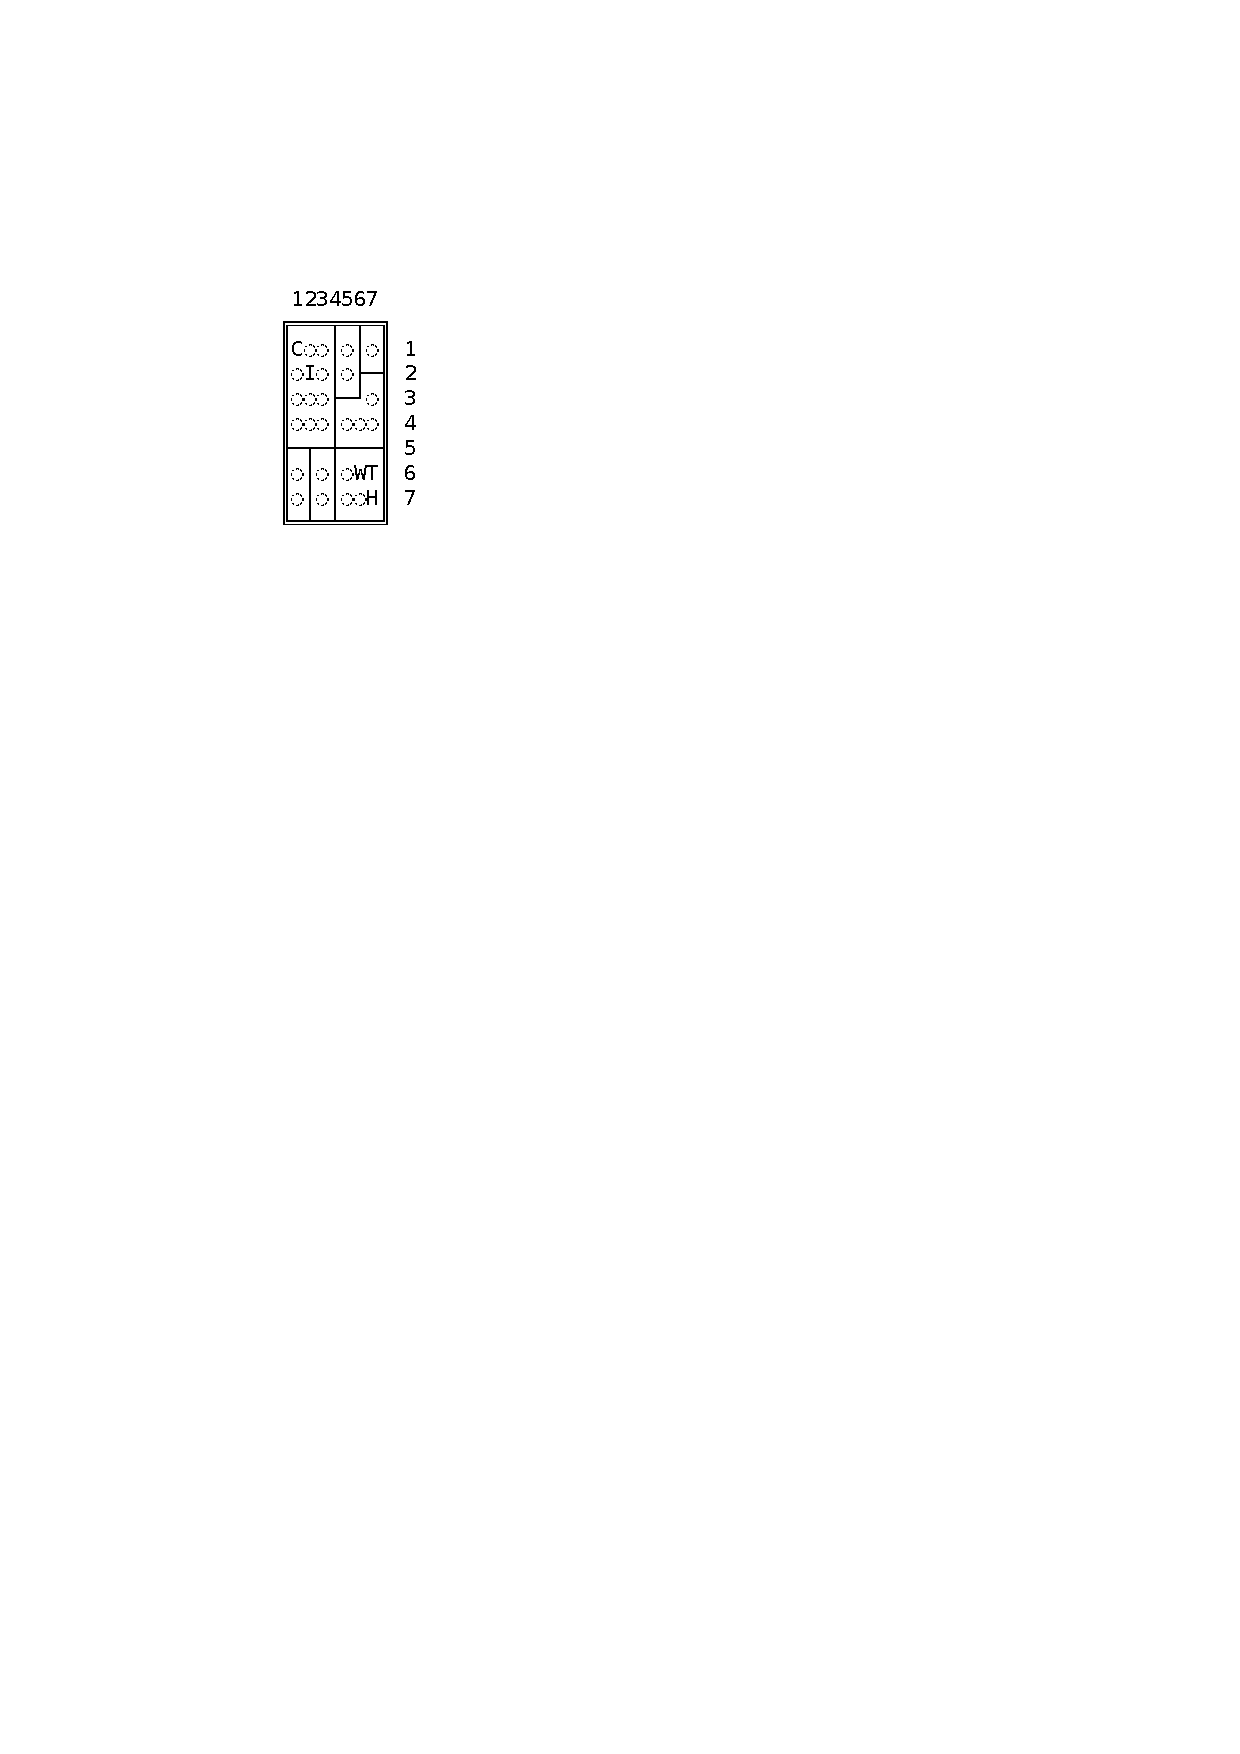
\includegraphics[height=60pt]{clean_up/grid_1_min.pdf}\\
                \raggedright
                \texttt{Please send a message to the other player to start the game!}
            }
        }
    }
    & \\

\theutterance \stepcounter{utterance}  
    & \multicolumn{4}{p{0.6\linewidth}}{
        \cellcolor[rgb]{0.561,0.737,0.561}{
            \makecell[{{p{\linewidth}}}]{
                \texttt{\tiny{[P1$\rangle$GM]}}
                \texttt{SAY: Hi! Let's coordinate our moves. [...]}
            }
        }
    }
    & & \\

\theutterance \stepcounter{utterance}  
    & & \multicolumn{4}{p{0.6\linewidth}}{
        \cellcolor[rgb]{0.9,0.9,0.9}{
            \makecell[{{p{\linewidth}}}]{
                \texttt{\tiny{[GM$\rangle$P2]}}
                \centering{<GAME DESCRIPTION>}\\
                \centering
                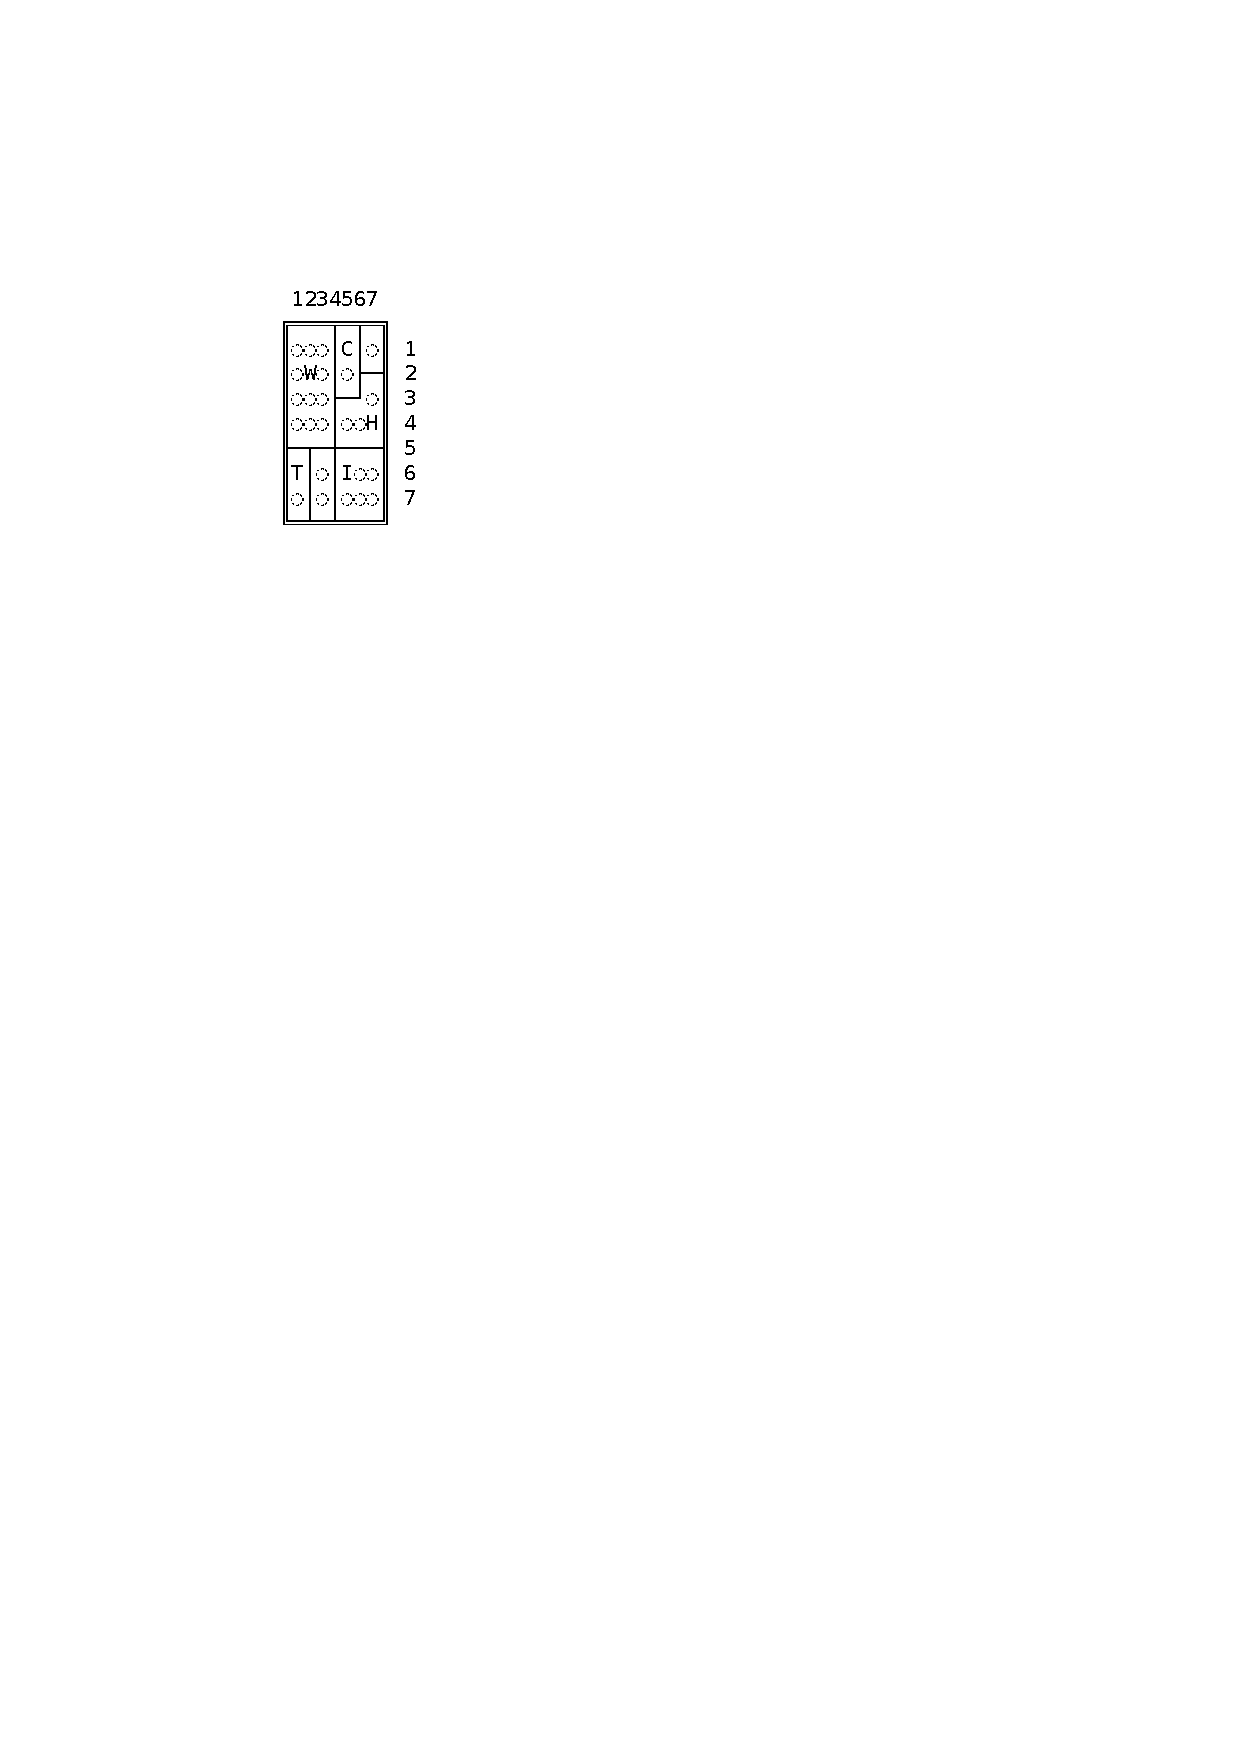
\includegraphics[height=60pt]{clean_up/grid_2_min.pdf}\\
                \raggedright
                \texttt{The other player started the game by sending this message:} \\
                \centering{<MESSAGE>}\\
                \raggedright
                \texttt{What is your first command?}
            }
        }
    }
    & \\

& \multicolumn{6}{c}{
\vdots
} \\

\theutterance \stepcounter{utterance}  
    & & & \multicolumn{4}{p{0.6\linewidth}}{
        \cellcolor[rgb]{0.373,0.62,0.627}{
            \makecell[{{p{\linewidth}}}]{
                \texttt{\tiny{[GM$\langle$P2]}}
                \texttt{MOVE: C, (1,1)} \\
            }
        }
    } \\

\theutterance \stepcounter{utterance}  
    & & \multicolumn{4}{p{0.6\linewidth}}{
        \cellcolor[rgb]{0.9,0.9,0.9}{
            \makecell[{{p{\linewidth}}}]{
                \texttt{\tiny{[P1$\langle$GM]}}
                Your message has been relayed to the other player.\\
                \centering <GAME STATE> \\
                \raggedright
                \texttt{The other player moved an object on their grid. \\What is your next command?}
            }
        }
    }
    & \\
    
\theutterance \stepcounter{utterance}  
    & \multicolumn{4}{p{0.6\linewidth}}{
        \cellcolor[rgb]{0.561,0.737,0.561}{
            \makecell[{{p{\linewidth}}}]{
                \texttt{\tiny{[P1$\rangle$GM]}}
                \texttt{MOVE: I, (5,6)}
            }
        }
    }
    & & \\

& \multicolumn{6}{c}{
    \vdots
} \\
\theutterance \stepcounter{utterance}  
    & & & \multicolumn{4}{p{0.6\linewidth}}{
        \cellcolor[rgb]{0.373,0.62,0.627}{
            \makecell[{{p{\linewidth}}}]{
                \texttt{\tiny{[GM$\langle$P2]}}
                \texttt{SAY: I think our grids are aligned now, finished?} \\
            }
        }
    } \\
\theutterance \stepcounter{utterance}  
    & \multicolumn{4}{p{0.6\linewidth}}{
        \cellcolor[rgb]{0.561,0.737,0.561}{
            \makecell[{{p{\linewidth}}}]{
                \texttt{\tiny{[P1$\rangle$GM]}}
                \texttt{SAY: finished!}
            }
        }
    }
    & & \\
\end{supertabular}
    \caption{Example episode from Clean Up game to achieve a common goal configuration for a number of objects randomly placed on each player`s grid, and move them accordingly. Finally, both players have to agree the goal is reached to end the game.}
    \vspace*{-.6cm}
    \label{fig:clean_up_example}
\end{figure}

\paragraph{Game Mechanics} Both players are presented with $7\times7$ ASCII grids, with a number of randomly distributed objects in the form of capital letters placed on them. In each turn, a player can either send a message to their counterpart or move an object on their grid. The message and move text require certain formatting rules to follow. If a player does not follow the format, tries to move an object to a non-empty space or outside the grid bounds, or tries to move an object that doesn't exist, they receive a penalty and are re-prompted with information on the nature of their mistake. The game ends if (1) both players agree to end it, (2) round limit is exceeded, or (3) penalty limit is exceeded.




\paragraph{Game Instances}

All instances are created programmatically by creating different grids ($7\times7$), which contain obstacles in form of horizontal and vertical lines, branches, crossings, and corners. The maximum number of rounds is fixed to $4 \times n_{obj}$ (where $n_{obj}$ is the object count). 
% Players can collectively accumulate $2 \times n_{obj} + 2$ penalties. 
We create different sets of experiments by controlling two aspects: number of empty cells and objects. We have three difficulty levels. Of the 49 total cells, $34$ of cells are empty on the \textit{easy}, $29$ on \textit{medium}, and $24$ on \textit{hard} levels. For each level, we sample three grids, and then place $3$, $5$, or $7$ objects on them, making for \textbf{27 instances in total}.

\begin{figure}[ht]
    \centering
    % \newcounter{utterance}
{\footnotesize  \setcounter{utterance}{1}
\setlength{\tabcolsep}{0pt}
\begin{supertabular}{c@{$\;$}|p{.15\linewidth}@{}p{.15\linewidth}p{.15\linewidth}p{.15\linewidth}p{.15\linewidth}p{.15\linewidth}}   
\# & $\;$A & \multicolumn{4}{c}{Game Master} & $\;\:$B\\
    \hline

\theutterance \stepcounter{utterance}  
    & & \multicolumn{4}{p{0.6\linewidth}}{
        \cellcolor[rgb]{0.9,0.9,0.9}{
            \makecell[{{p{\linewidth}}}]{
                \texttt{\tiny{[A$\langle$GM]}}
                <GAME DESCRIPTION>\\
                \texttt{-Items and weights: Ball(2), Book(3), Magazine(1), Rope(4), Lamp(5)} \\
                \texttt{-Max Weight: 7} \\
                \texttt{-Your Preferences: Ball=1, Book=2, Magazine=2, Rope=2, Lamp=1}
            }
        }
    }
    & \\
    
\theutterance \stepcounter{utterance}  
    & \multicolumn{4}{p{0.6\linewidth}}{
        \cellcolor[rgb]{1,0.9,0.9}{
            \makecell[{{p{\linewidth}}}]{
                \texttt{\tiny{[A$\rangle$GM]}}
                \texttt{PROPOSAL: Magazine, Ball, Book} \\
                \texttt{ARGUMENT: These items balance weight and value well for me. What do you think?}
            }
        }
    }
    & & \\

\theutterance \stepcounter{utterance}  
    & & \multicolumn{4}{p{0.6\linewidth}}{
        \cellcolor[rgb]{0.9,0.9,0.9}{
            \makecell[{{p{\linewidth}}}]{
                \texttt{\tiny{[GM$\rangle$B]}}
                <GAME DESCRIPTION>\\
                \texttt{<Items, weights, weight limit>}\\
                \texttt{-Your Preferences: Ball=1, Book=1, Magazine=2, Rope=4, Lamp=5} \\
                \centering{<PLAYER A Message>}
            }
        }
    }
    & \\

\theutterance \stepcounter{utterance}  
    & & & \multicolumn{4}{p{0.6\linewidth}}{
        \cellcolor[rgb]{0.9,1,0.9}{
            \makecell[{{p{\linewidth}}}]{
                \texttt{\tiny{[GM$\langle$B]}}
                \texttt{PROPOSAL: Rope, Ball, Magazine}\\
                \texttt{ARGUMENT: I value Rope highly, but not Magazine. How about we swap them?}
            }
        }
    } \\

\theutterance \stepcounter{utterance}  
    & & \multicolumn{4}{p{0.6\linewidth}}{
        \cellcolor[rgb]{0.9,0.9,0.9}{
            \makecell[{{p{\linewidth}}}]{
                \texttt{\tiny{[A$\langle$GM]}}
                \centering{<PLAYER B Message>}
            }
        }
    }
    & \\

\theutterance \stepcounter{utterance}  
    & \multicolumn{4}{p{0.6\linewidth}}{
        \cellcolor[rgb]{1,0.9,0.9}{
            \makecell[{{p{\linewidth}}}]{
                \texttt{\tiny{[A$\rangle$GM]}}
                \texttt{AGREE: Rope, Ball, Magazine} \\
                \texttt{ARGUMENT: I am indifferent w.r.t. Rope and Magazine. Fair deal.} \\
            }
        }
    }
    & & \\
    
\end{supertabular}
}
    \caption{An example episode of the \textit{Air Balloon Survival} game. Two players must negotiate and argue for their preferred set of items. and must explicitly agree to a proposal made by the other.}
    \label{fig:air_balloon_example}
    \vspace*{-.6cm}
\end{figure}

\subsection{Air Balloon Survival}
This game evaluates advanced reasoning and interactive collaboration between players, which was previously introduced by \citet{howes2021justifiable} to study how patients with schizophrenia verbalise their reasoning during social encounters. In our version, two players are on a sinking hot air balloon, and they have to agree on which items to keep (or throw out) so that the weight of the balloon is reduced to keep floating. Each player has hidden preference values for items and must negotiate to maximise their combined utility score. An example episode is given in Figure~\ref{fig:air_balloon_example}. The game tests individual reasoning through constraint-based optimisation, requiring arithmetic and combinatorial search, collective reasoning through practical rationality, and theory of mind (to infer their counterpart's hidden preferences from their responses to reach an optimal agreement). We provide all prompts and other details in Appendix~\ref{sec:appendix_airballoon}.


\paragraph{Game Mechanics}
Both players receive their assigned preference values for the items. They are instructed to use specified formats when making proposals and engaging in negotiations. The game is aborted if no progress is made for eight consecutive turns. 
% Each player may make up to two mistakes (either by violating game rules or the required syntax). 
Unlike the other two games, players are also instructed to output their \texttt{STRATEGIC REASONING} along with the expected message. Only the expected message is passed to the other player. It allows players to ``think out loud'' about their choices. The game ends when a proposal made by one player is accepted by the other.

\paragraph{Instance Generation}

We draw either $15$ or $35$ items (depending on the experiment) from a randomly generated list constructed by concatenating a capital letter with a two-digit number (e.g., \texttt{A42}, \texttt{C07})\footnote{This keeps the naming of items language-agnostic and abstract from conventional examples of the \textit{0/1 Knapsack Problem} models that may have been seen during training}. We assign a weight value to each item. The air balloon's capacity is defined as a fraction of the combined weight of all items. We experiment with two negotiation levels, where we specifically set valuations over items to be the same for players, giving them common goals (easy level), or we invert their preference orderings, giving them opposing goals (hard level). We also experiment with generating the \texttt{STRATEGIC REASONING} or not. Lastly, we conduct complexity experiments by increasing the number of items. In total, we have six experiments with each having six instances, which leads to the \textbf{total number of 36 instances} for this game.



\section{Experimental Setup}\label{sec:experimental_setup}

\subsection{Game Instances}

\textit{Deal or No Deal}, \textit{Clean Up}, and \textit{Air Balloon Survival} games include 40, 27, and 36 experimental instances, respectively. Each instance is then initialised with defined prompt templates. The same game instances are used for the English, German, and Italian experiments because the instances are language-agnostic; only the prompt templates need to be aligned for a specific language. 

%All prompt templates are provided in Appendix \ref{sec:dond_prompt_templates}, \ref{clean_up:prompts}, \ref{sec:hot_air_balloon_appendix_prompt_templates}.


\subsection{Evaluation Metrics}

The \textit{clembench framework}~\cite{chalamalasetti-etal-2023-clembench} requires each implemented game to provide two primary metrics: \% Played and Quality Score. The \textit{\% Played} stands for the percentage of episodes where the evaluated language models followed instructions and the game was terminated by the defined end states. In cases where the gameplay does not fit the defined states of the game, the Game Master either tolerates such behaviour for one or two turns, asks the players to try again, or aborts the game. The \textit{Quality Score} is calculated using an objective function to measure how closely the played episode aligns with the target goal. In each game, this metric is calculated for all episodes that have been played. Once two metrics are calculated, they are aggregated to a single number, the \textit{clemscore} as the normalised product of \textit{\% Played} and \textit{Quality Score} (scaled to the interval [0, 100]). Next, we describe the Quality Scores for games.

\paragraph{Deal or No Deal}

For the cooperative game mode, we measure quality as the ratio of achieved total score to maximum possible total score. For the semi-competitive setting, we use a \textit{Pareto efficiency} metric that measures how far the agreement is from optimal by calculating potential one-sided improvements (more details in Appendix~\ref{subsec:appendix_dond_metric}).

\paragraph{Clean Up}

The Quality Score combines two main components: how well players organised objects spatially and how many rule violations they incurred. The metric uses \textit{Euclidean distances} between matching objects to compare the final arrangement to both the initial setup and a random baseline, rewarding improvements in object alignment while penalising rule violations through a scaling factor that becomes increasingly harsh as violations approach the maximum allowed limit 
(more details in Appendix~\ref{subsec:appendix_cleanup_evaluation_metric}).

\begin{table*}[ht]
\centering
\footnotesize
\setlength{\tabcolsep}{4.5pt}
\definecolor{lightgreen}{RGB}{220,255,220}
\definecolor{lightblue}{RGB}{220,235,255}
\definecolor{darkgreen}{rgb}{0.0, 0.5, 0.0}
\definecolor{darkred}{rgb}{0.8, 0.0, 0.0}
% The '|' between the last two 'c's ensures the line appears in data rows by default
\begin{tabular}{c|l|cc|cc|cc|cc|cc|cc|c|c} 
\multirow{9}{*}{\rotatebox{90}{\textbf{EN}}} & & \multicolumn{2}{c}{\textbf{GPT-5}} & \multicolumn{2}{c}{\begin{tabular}{c}\textbf{GPT-5}\\\textbf{mini}\end{tabular}} & \multicolumn{2}{c}{\textbf{CL-4}} & \multicolumn{2}{c}{\textbf{LM-70B}} & \multicolumn{2}{c}{\textbf{Nem-9B}} & \multicolumn{2}{c}{\textbf{Qwen-3}} & 
% This \multicolumn overrides the default and removes the vertical line for this cell only
\multicolumn{1}{c}{\begin{tabular}{c}\textbf{GPT}\\\textbf{OSS}\end{tabular}} & \textbf{DS-v3.1} \\ \cline{2-16}

& \textbf{Games} & On & Off & On & Off & On & Off & On & Off & On & Off & On & Off & On & Off \\ \hline
 & DoND & \cellcolor{lightgreen}87.9 & \cellcolor{lightblue}32.3 & \cellcolor{lightgreen}75.7 & \cellcolor{lightblue}23.7 & \cellcolor{lightgreen}\textbf{94.4} & \cellcolor{lightblue}90.1 & \cellcolor{lightgreen}24.3 & \cellcolor{lightblue}43.5 & \cellcolor{lightgreen}18.5 & \cellcolor{lightblue}4.0 & \cellcolor{lightgreen}57.9 & \cellcolor{lightblue}22.5 & \cellcolor{lightgreen}50.0 & \cellcolor{lightblue}59.0 \\ 
 & Clean Up & \cellcolor{lightgreen}\textbf{99.8} & \cellcolor{lightblue}75.2 & \cellcolor{lightgreen}96.6 & \cellcolor{lightblue}77.3 & \cellcolor{lightgreen}85.5 & \cellcolor{lightblue}81.9 & \cellcolor{lightgreen}4.1 & \cellcolor{lightblue}28.1 & \cellcolor{lightgreen}28.5 & \cellcolor{lightblue}35.1 & \cellcolor{lightgreen}87.9 & \cellcolor{lightblue}35.8 & \cellcolor{lightgreen}81.4 & \cellcolor{lightblue}76.4 \\ 
 & Air Balloon & \cellcolor{lightgreen}\textbf{98.0} & \cellcolor{lightblue}80.1 & \cellcolor{lightgreen}97.5 & \cellcolor{lightblue}82.2 & \cellcolor{lightgreen}83.8 & \cellcolor{lightblue}26.2 & \cellcolor{lightgreen}2.3 & \cellcolor{lightblue}40.9 & \cellcolor{lightgreen}14.3 & \cellcolor{lightblue}13.2 & \cellcolor{lightgreen}88.7 & \cellcolor{lightblue}0 & \cellcolor{lightgreen}78.2 & \cellcolor{lightblue}81.7 \\ 
 & \textbf{Average} & \cellcolor{lightgreen}\textbf{95.2} & \cellcolor{lightblue}62.5 & \cellcolor{lightgreen}89.9 & \cellcolor{lightblue}61.1 & \cellcolor{lightgreen}87.9 & \cellcolor{lightblue}66.1 & \cellcolor{lightgreen}10.2 & \cellcolor{lightblue}37.5 & \cellcolor{lightgreen}20.4 & \cellcolor{lightblue}17.4 & \cellcolor{lightgreen}78.2 & \cellcolor{lightblue}19.4 & \cellcolor{lightgreen}69.9 & \cellcolor{lightblue}72.4 \\ 
& \textbf{Margin} & \multicolumn{2}{c|}{\textcolor{darkgreen}{+32.7}} & \multicolumn{2}{c|}{\textcolor{darkgreen}{+28.8}} & \multicolumn{2}{c|}{\textcolor{darkgreen}{+21.8}} & \multicolumn{2}{c|}{\textcolor{darkred}{-27.3}} & \multicolumn{2}{c|}{\textcolor{darkgreen}{+3.0}} & \multicolumn{2}{c|}{\textcolor{darkgreen}{+58.8}} & - & -\\ \hline \hline

 
\multirow{4}{*}{\rotatebox{90}{\textbf{DE}}}
 & DoND & \cellcolor{lightgreen}\textbf{86.0} & \cellcolor{lightblue}19.6 & \cellcolor{lightgreen}82.9 & \cellcolor{lightblue}24.4 & \cellcolor{lightgreen}80.3 & \cellcolor{lightblue}77.1 & \cellcolor{lightgreen}21.8 & \cellcolor{lightblue}53.4 & \cellcolor{lightgreen}0 & \cellcolor{lightblue}4.5 & \cellcolor{lightgreen}62.1 & \cellcolor{lightblue}12.8 & \cellcolor{lightgreen}34.9 & \cellcolor{lightblue}42.4 \\ 
 & Clean Up & \cellcolor{lightgreen}98.2 & \cellcolor{lightblue}70.4 & \cellcolor{lightgreen}\textbf{98.8} & \cellcolor{lightblue}67.0 & \cellcolor{lightgreen}94.3 & \cellcolor{lightblue}83.1 & \cellcolor{lightgreen}5.3 & \cellcolor{lightblue}25.3 & \cellcolor{lightgreen}23.1 & \cellcolor{lightblue}0 & \cellcolor{lightgreen}86.4 & \cellcolor{lightblue}27.5 & \cellcolor{lightgreen}74.4 & \cellcolor{lightblue}53.7 \\ 
 & Air Balloon & \cellcolor{lightgreen}\textbf{98.0} & \cellcolor{lightblue}81.4 & \cellcolor{lightgreen}94.9 & \cellcolor{lightblue}86.2 & \cellcolor{lightgreen}85.4 & \cellcolor{lightblue}27.8 & \cellcolor{lightgreen}51.5 & \cellcolor{lightblue}43.7 & \cellcolor{lightgreen}17.4 & \cellcolor{lightblue}16.3 & \cellcolor{lightgreen}76.0 & \cellcolor{lightblue}8.8 & \cellcolor{lightgreen}90.7 & \cellcolor{lightblue}75.3 \\ 
 & \textbf{Average} & \cellcolor{lightgreen}\textbf{94.1} & \cellcolor{lightblue}57.1 & \cellcolor{lightgreen}92.2 & \cellcolor{lightblue}59.2 & \cellcolor{lightgreen}86.7 & \cellcolor{lightblue}62.7 & \cellcolor{lightgreen}26.2 & \cellcolor{lightblue}40.8 & \cellcolor{lightgreen}13.5 & \cellcolor{lightblue}6.9 & \cellcolor{lightgreen}74.8 & \cellcolor{lightblue}16.4 & \cellcolor{lightgreen}66.7 & \cellcolor{lightblue}57.1 \\
& \textbf{Margin} & \multicolumn{2}{c|}{\textcolor{darkgreen}{+37.0}} & \multicolumn{2}{c|}{\textcolor{darkgreen}{+33.0}} & \multicolumn{2}{c|}{\textcolor{darkgreen}{+24.0}} & \multicolumn{2}{c|}{\textcolor{darkred}{-14.6}} & \multicolumn{2}{c|}{\textcolor{darkgreen}{+6.6}} & \multicolumn{2}{c|}{\textcolor{darkgreen}{+58.4}} & - & - \\ \hline \hline

 
\multirow{4}{*}{\rotatebox{90}{\textbf{IT}}}
 & DoND & \cellcolor{lightgreen}78.0 & \cellcolor{lightblue}33.8 & \cellcolor{lightgreen}77.1 & \cellcolor{lightblue}26.8 & \cellcolor{lightgreen}\textbf{84.4} & \cellcolor{lightblue}67.8 & \cellcolor{lightgreen}17.3 & \cellcolor{lightblue}14.3 & \cellcolor{lightgreen}13.9 & \cellcolor{lightblue}11.2 & \cellcolor{lightgreen}55.6 & \cellcolor{lightblue}19.4 & \cellcolor{lightgreen}29.0 & \cellcolor{lightblue}28.9 \\ 
 & Clean Up & \cellcolor{lightgreen}89.0 & \cellcolor{lightblue}68.8 & \cellcolor{lightgreen}\textbf{93.6} & \cellcolor{lightblue}77.2 & \cellcolor{lightgreen}91.6 & \cellcolor{lightblue}82.6 & \cellcolor{lightgreen}6.5 & \cellcolor{lightblue}31.1 & \cellcolor{lightgreen}21.5 & \cellcolor{lightblue}12.7 & \cellcolor{lightgreen}82.6 & \cellcolor{lightblue}31.5 & \cellcolor{lightgreen}63.6 & \cellcolor{lightblue}67.6 \\ 
 & Air Balloon & \cellcolor{lightgreen}97.2 & \cellcolor{lightblue}88.0 & \cellcolor{lightgreen}\textbf{97.3} & \cellcolor{lightblue}87.8 & \cellcolor{lightgreen}79.4 & \cellcolor{lightblue}27.0 & \cellcolor{lightgreen}2.7 & \cellcolor{lightblue}40.8 & \cellcolor{lightgreen}0 & \cellcolor{lightblue}0 & \cellcolor{lightgreen}77.8 & \cellcolor{lightblue}12.9 & \cellcolor{lightgreen}83.7 & \cellcolor{lightblue}76.4 \\ 
 & \textbf{Average} & \cellcolor{lightgreen}88.1 & \cellcolor{lightblue}63.5 & \cellcolor{lightgreen}\textbf{89.3} & \cellcolor{lightblue}63.9 & \cellcolor{lightgreen}85.1 & \cellcolor{lightblue}59.1 & \cellcolor{lightgreen}8.8 & \cellcolor{lightblue}28.7 & \cellcolor{lightgreen}11.8 & \cellcolor{lightblue}8.0 & \cellcolor{lightgreen}72.0 & \cellcolor{lightblue}21.3 & \cellcolor{lightgreen}58.8 & \cellcolor{lightblue}57.6 \\
 & \textbf{Margin} & \multicolumn{2}{c|}{\textcolor{darkgreen}{+24.6}} & \multicolumn{2}{c|}{\textcolor{darkgreen}{+25.4}} & \multicolumn{2}{c|}{\textcolor{darkgreen}{+26.0}} & \multicolumn{2}{c|}{\textcolor{darkred}{-19.9}} & \multicolumn{2}{c|}{\textcolor{darkgreen}{+3.8}} & \multicolumn{2}{c|}{\textcolor{darkgreen}{+50.7}} & - & - \\ \hline
\hline

\multicolumn{2}{c|}{\textbf{Overall Average}} & \cellcolor{lightgreen}\textbf{92.5} & \cellcolor{lightblue}61.1 & \cellcolor{lightgreen}90.5 & \cellcolor{lightblue}61.4 & \cellcolor{lightgreen}86.6 & \cellcolor{lightblue}62.6 & \cellcolor{lightgreen}15.1 & \cellcolor{lightblue}35.7 & \cellcolor{lightgreen}15.2 & \cellcolor{lightblue}10.8 & \cellcolor{lightgreen}75.0 & \cellcolor{lightblue}19.0 & \cellcolor{lightgreen}65.1 & \cellcolor{lightblue}62.4 \\
\multicolumn{2}{c|}{\textbf{Overall Margin}} & \multicolumn{2}{c|}{\textcolor{darkgreen}{+31.4}} & \multicolumn{2}{c|}{\textcolor{darkgreen}{+29.1}} & \multicolumn{2}{c|}{\textcolor{darkgreen}{+24.0}} & \multicolumn{2}{c|}{\textcolor{darkred}{-20.6}} & \multicolumn{2}{c|}{\textcolor{darkgreen}{+4.4}} & \multicolumn{2}{c|}{\textcolor{darkgreen}{+56.0}} & - & - \\ \hline

\end{tabular}
\caption{\textit{clemscore} values for three negotiation games on selected LLMs for English, German, and Italian versions. \textit{On}: reasoning mode is turned on, \textit{Off}: reasoning mode is turned off. The best result for each language in each row is highlighted in bold. \textit{CL}: Claude, \textit{LM}: Llama-3.3, \textit{DS}: Deepseek, \textit{Nem}: Nemotron-v2, \textit{DoND}: Deal or No Deal }
\label{tab:main-results}
\end{table*}




\paragraph{Air Balloon Survival}

Each player receives a score based on their achieved utility relative to their optimal knapsack solution. The overall game score uses the harmonic mean of both players' normalised scores, which rewards balanced outcomes and penalises deals where one player benefits disproportionately (more details in Appendix~\ref{subsec:appendix_balloon_metrics}).

\subsection{Evaluated Models}

We have evaluated both commercial and open-weight models that have reasoning functionality. We selected \textit{GPT-5}, \textit{GPT-5-mini}, \textit{Claude-4} from commercial models. From open-weight models, we selected \textit{Llama3.3-70B} and \textit{Deepseek-R1-distilled-llama-70B} as its reasoning counterpart\footnote{Llama3.3-70B model was finetuned to make it a reasoning model by distilling from Deepseek-R1}, \textit{Nemotron-Nano-9B-v2}, \textit{Qwen-3-80B} (\textit{instruction} and \textit{thinking} versions for reasoning off and on modes, respectively), \textit{GPT-OSS-120B} with reasoning on mode, and finally \textit{Deepseek-v3.1} with reasoning off mode. For commercial models, we ran them via their respective API backends, and we used \textit{OpenRouter.ai} for open-weight models.


\section{Results}

\subsection{Overall Performance}

\begin{figure*}[ht]
    \centering
    \begin{subfigure}[b]{0.49\textwidth}
        \centering
        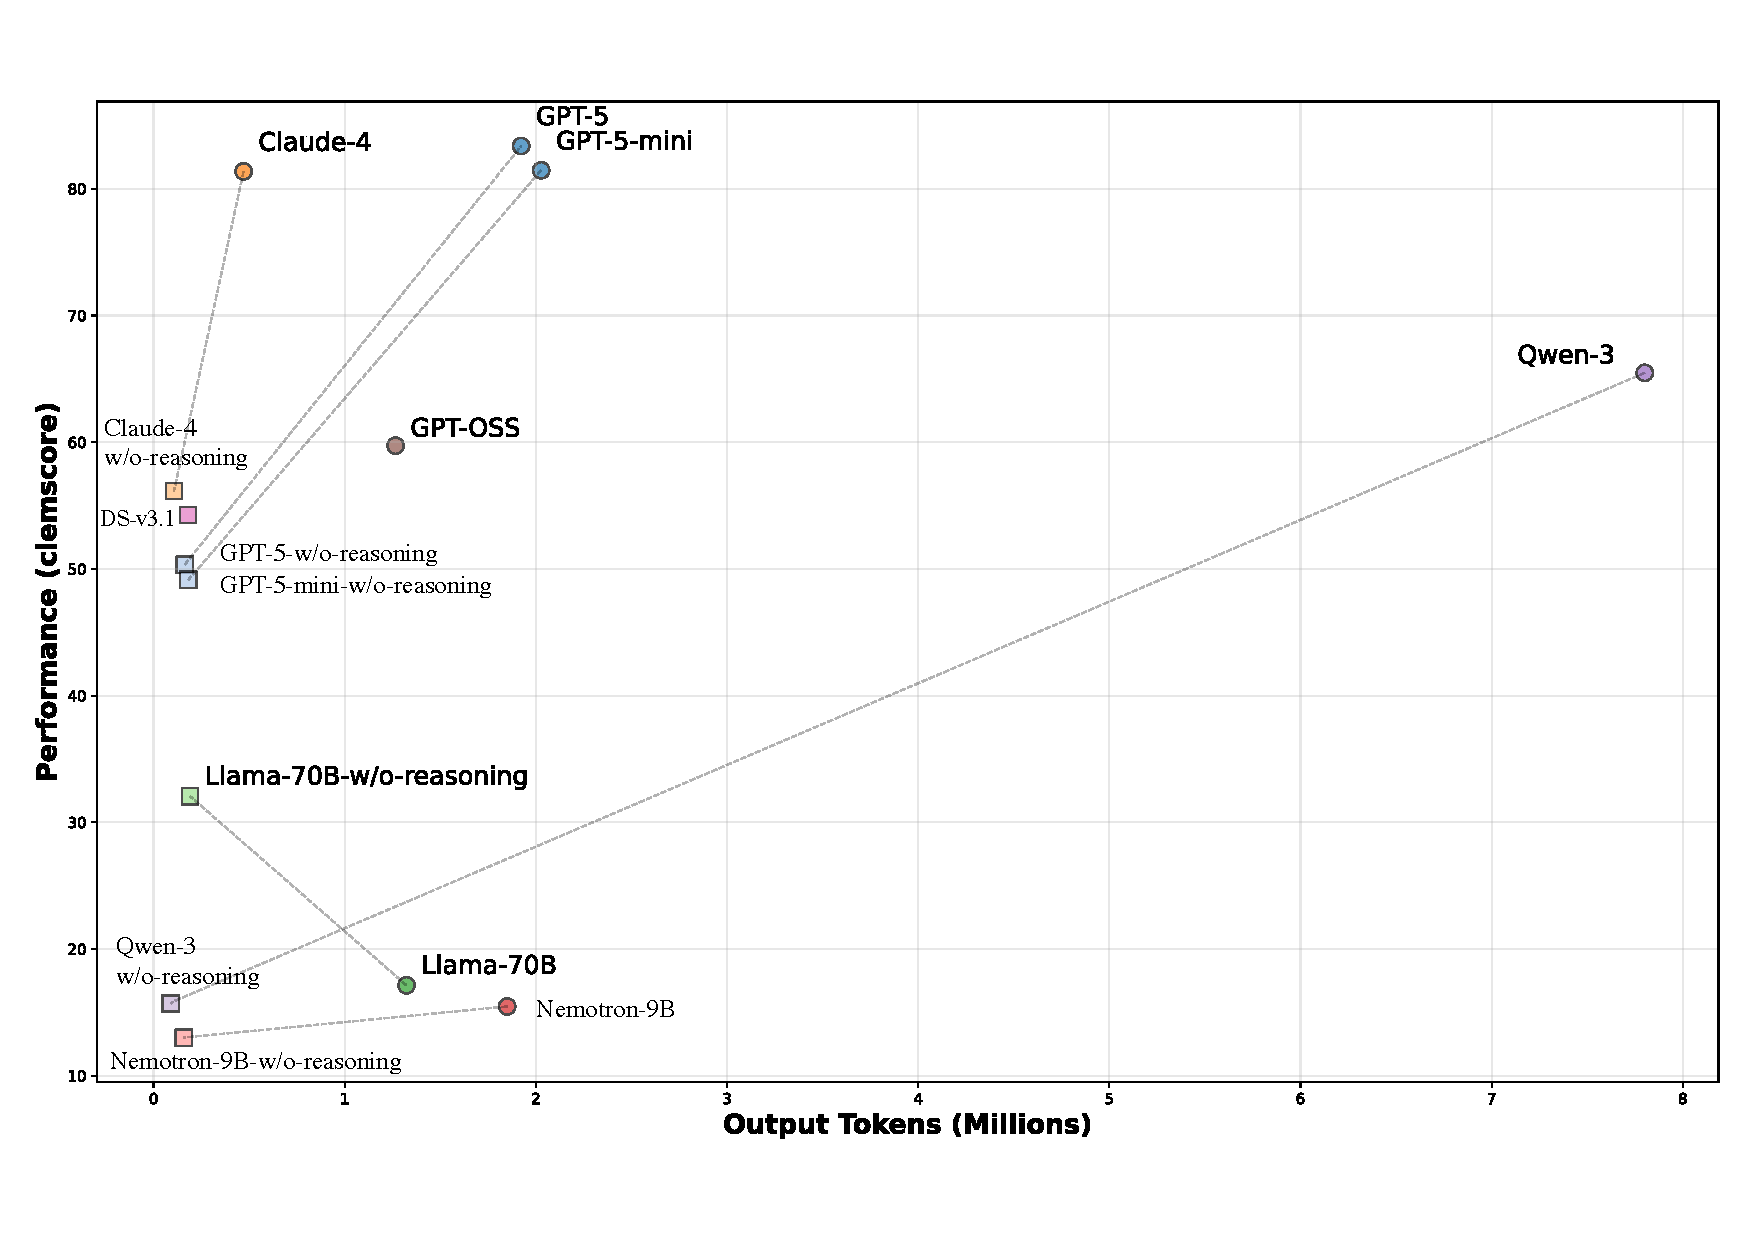
\includegraphics[width=\linewidth]{figures/output_token_plot_average.pdf}
        \caption{Performance and the output tokens for all evaluated models with their reasoning on/off modes averaged for three languages.}
        \label{fig:token_average}
    \end{subfigure}
    \hfill
    \begin{subfigure}[b]{0.49\textwidth}
        \centering
        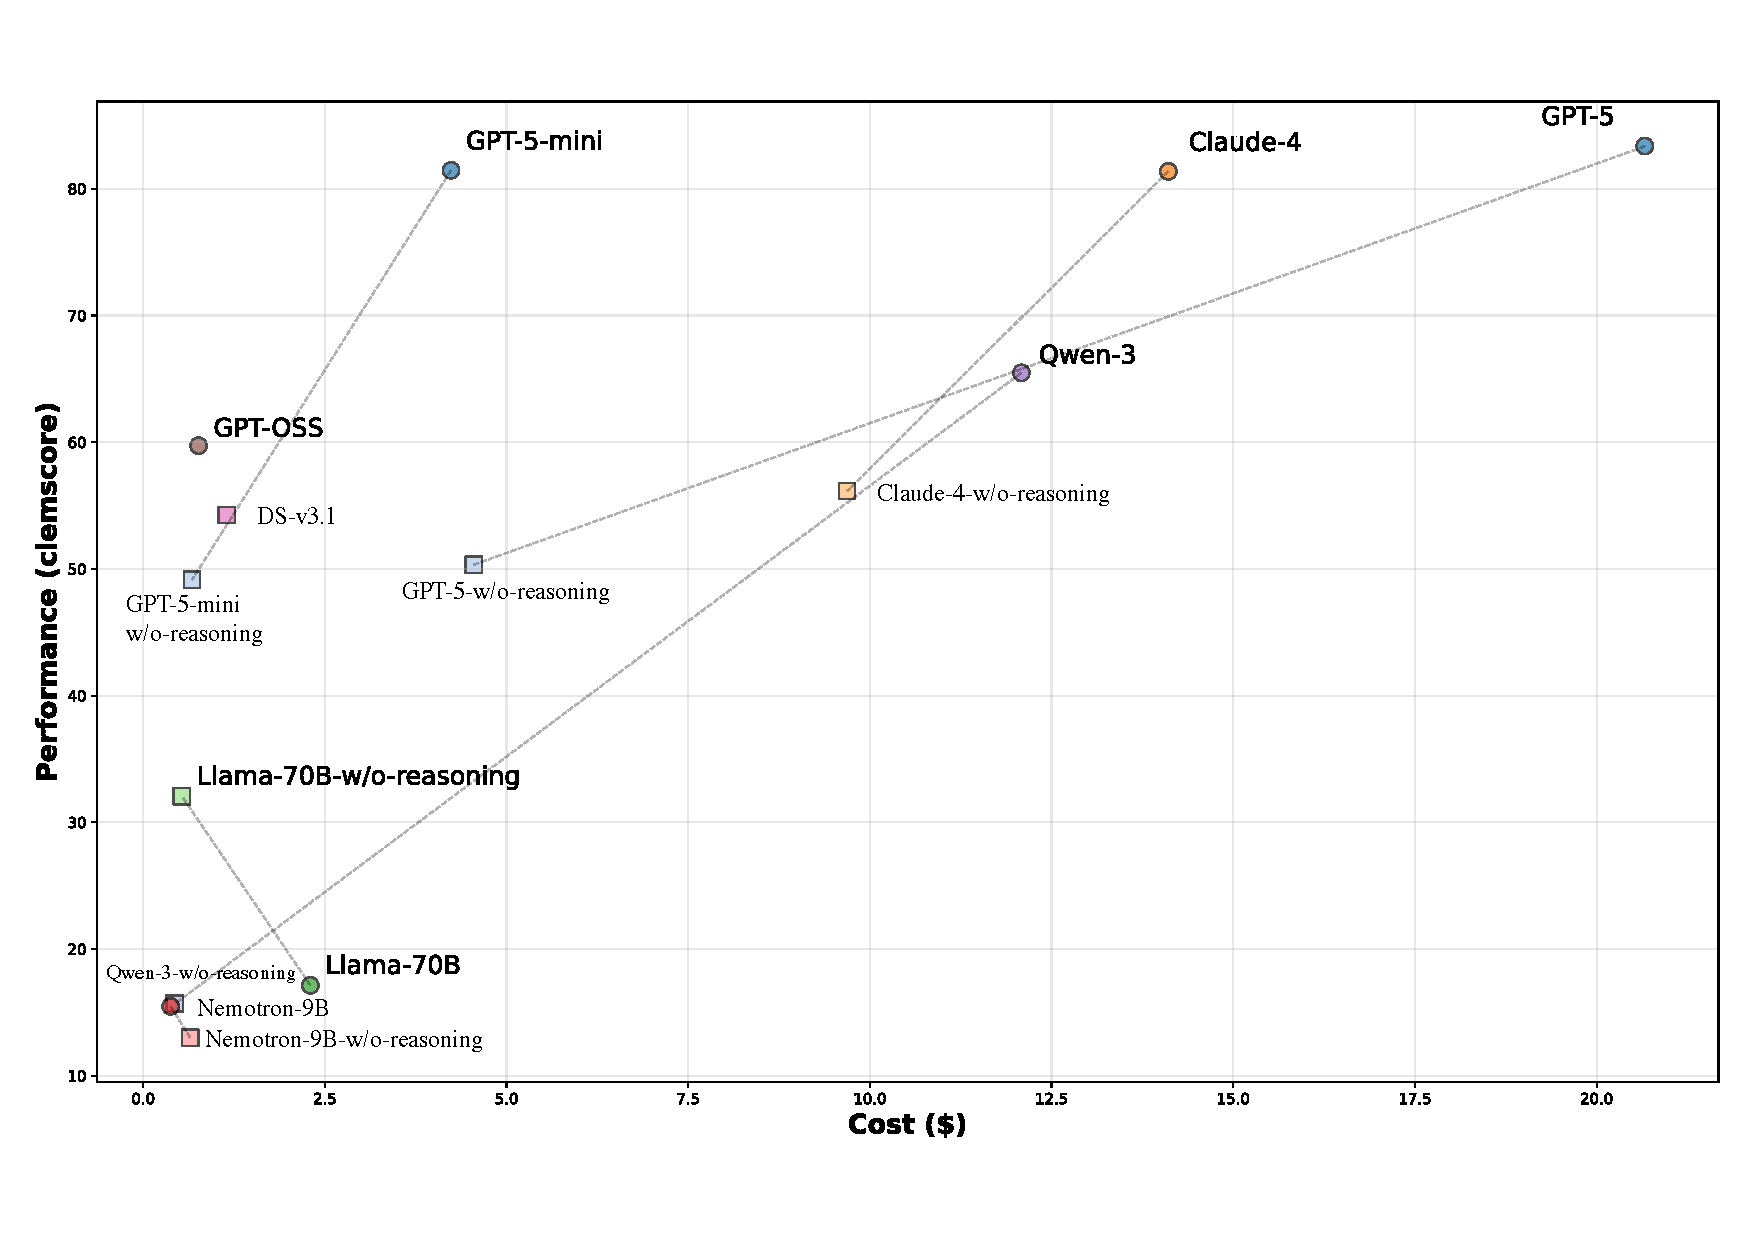
\includegraphics[width=\linewidth]{figures/cost_plot_average.pdf}
        \caption{Performance and the cost of for all evaluated models with their reasoning on/off modes averaged for three languages.}
        \label{fig:cost_average}
    \end{subfigure}
    \caption{Trade-off between performance and cost comparison averaged across languages.}
    \label{fig:combined-token-cost}
    \vspace{-1.2em} % desperate times
\end{figure*}

We present the results obtained by the models (in \textit{reasoning on} and \textit{off} modes, where possible) evaluated for the English, German, and Italian versions of the negotiation game in Table~\ref{tab:main-results}. 
% \textit{GPT-OSS} (reasoning on) and \textit{Deepseek-v3.1} (reasoning off) were run in one mode only due to their underlying architecture.

\textbf{The Effect of Reasoning}: the most striking observation here is that reasoning mode dramatically improves performance across many models and languages, with \textit{Qwen-3} gaining $56$ points averaged across all games. Similar pattern exists for \textit{GPT}, \textit{Claude} and even smaller \textit{Nemotron} models. This is a strong indication that deliberate reasoning significantly enhances strategic game-playing abilities. Only with \textit{Llama-70B} do we see different results, which may be due to the effect of distillation.

\textbf{Multilingual Capabilities}: results for German shows the largest average margin between \textit{reasoning on} and \textit{off} modes of models. English and Italian performances are also strong, suggesting that certain models have particularly sufficient negotiation capabilities across these evaluated languages.

\textbf{Model Comparison}: GPT-5 is the clear winner, with GPT-5-mini and Claude-4 getting very close performance across all languages. Interestingly, GPT-5 mini sometimes matches or exceeds full GPT-5 performance (particularly in Italian). \textit{Qwen-3} shows the biggest performance jump.

\subsection{Detailed Analysis}


\textbf{RQ1}: \textit{What is the computational and performance trade-off between reasoning overhead and negotiation effectiveness across tasks and languages?}

In Figure~\ref{fig:combined-token-cost}~$a$, we present a plot that shows the average performance across all games and languages and how many output tokens it requires. Here, all reasoning and completion tokens are summed up. Most models generate the number of tokens that are closer to each other, and \textit{Qwen-3} generates almost \textit{4x} more tokens than others.

\begin{figure}[ht]
    \centering
    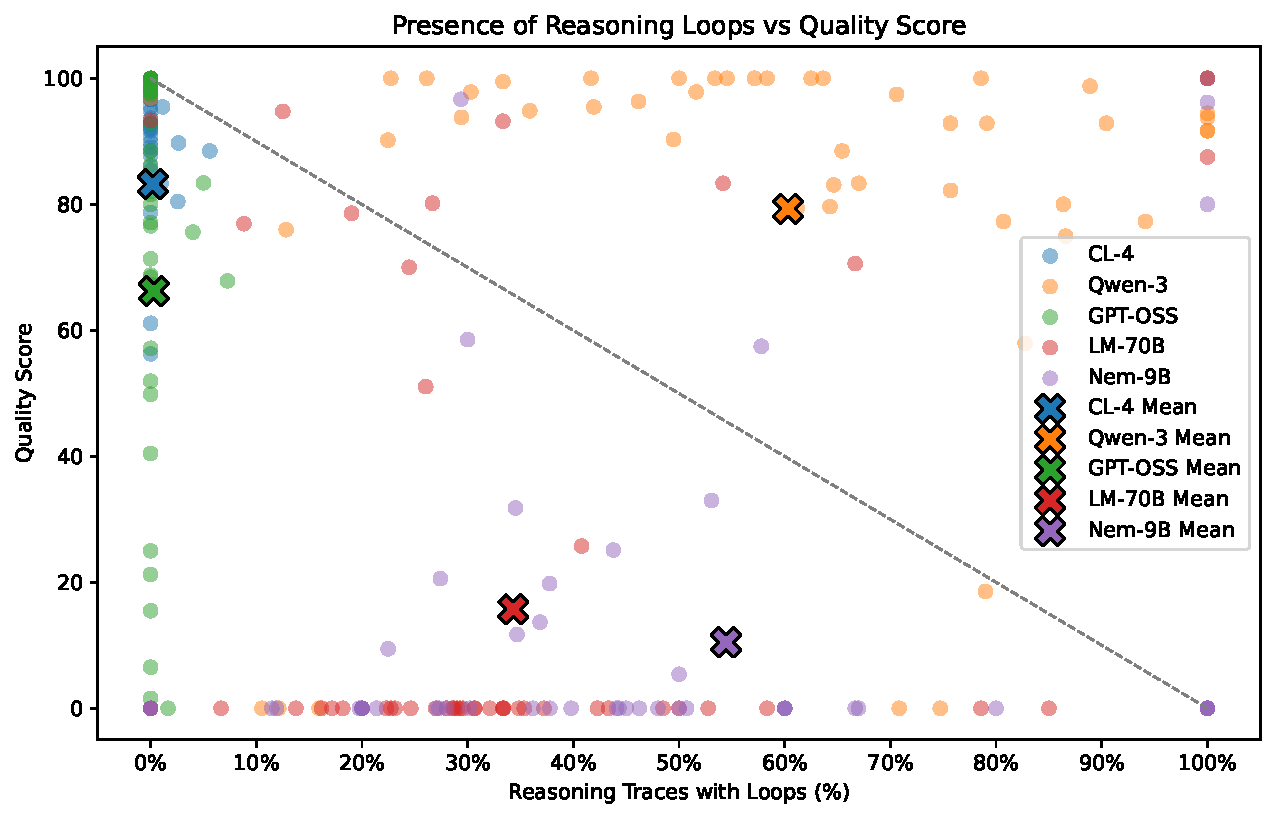
\includegraphics[width=\linewidth]{figures/loops_vs_quality_score.pdf}
    \caption{Reasoning traces that display thinking loops (at least three repetitions of the same action) plotted}
    \label{fig:reasoning_loops}
    \vspace{-1.2em}
\end{figure}

In Figure~\ref{fig:combined-token-cost}~$b$, we present the overall cost (input and output tokens together) of experiments for each model. As expected, models with reasoning mode cost more, with \textit{GPT-5}, being the most expensive, costing almost \textit{4x} compared to non-reasoning version while improving $31.4$ points in clemscore. In terms of deciding on the best trade-off between performance and cost, \textbf{\textit{GPT-5-mini} is the most cost-efficient commercial model, and \textit{GPT-OSS} is the best open-weight one, with a fraction of the cost compared to Qwen-3}.



We employed an LLM-based analysis to identify loops in 309 sampled transcripts. We prompted \textit{GPT-5} to classify the reasoning tokens of other models to check if there are any loops, which are actions or thoughts that are repeated at least three times (see Appendix~\ref{sec:llm-based_reasoning_analysis}). Figure~\ref{fig:reasoning_loops} shows the results for these transcripts. Good-performing model results should be clustered around top left, including fewer loops and high quality score. \textit{Claude-4} and \textit{GPT-OSS} rarely display loops (0.2\% and 0.3\%) and achieve high scores, while \textit{Llama-70B} (34.3\%) and \textit{Nemotron-9B} (54.4\%) contain loops and score low. 95.18\% of data points for these models fall below the dotted diagonal, indicating that reasoning loops, or \textit{overthinking} \cite{DBLP:journals/corr/abs-2506-06941}, reduce performance.
Conversely, \textit{Qwen-3} shows 60.3\% of traces with loops but averages 79.3 quality score. These excessive loops explain \textit{Qwen-3}'s high token counts.



% Additionally, we employed an LLM-based analysis to identify the percentage of reasoning traces containing loops, where an action or thought is repeated at least three times, in 309 sampled transcripts, see \ref{sec:llm-based_reasoning_analysis}. Fig.~\ref{fig:reasoning_loops} shows the percentage of reasoning traces containing loops in the transcripts on the x-axis and the quality score on the y-axis for these analysed transcripts. 
% Strikingly, Claude-4 and GPT-OSS virtually never display loops in their traces (0.2\% and 0.3\%) and achieve high scores, whereas 34.3\% of the reasoning traces of Llama-70B and 54.4\% of Nemotron-9B contain loops and achieve low scores. An overwhelming majority of 95.18\% of data points for these models are below the dotted diagonal, indicating that reasoning loops, a behaviour also known as \textit{overthinking} \cite{DBLP:journals/corr/abs-2506-06941}, tend to reduce performance.

% Perplexingly, the picture is reversed for Qwen-3, where 60.3\% of traces contain loops, but the average quality score for these instances is at 79.3, and 75\% of data points are above the diagonal. 
% Manual annotation of the last reasoning trace in a transcript for the hardest Clean Up experiment\footnote{Namely instance 1 of `2\_hard\_7obj\_en'.} revealed that the model tried to parse the current grid no less than 19 times, and additionally five times the initial grid, which has lost all relevance at this point. Still the model eventually reaches the conclusion that \textit{`probably multiple objects are already in place'} and opts to finish the game, reaching a Quality Score of 82.2. The high frequency of unnecessary loops is thus also the main reason for the extremely high numbers of output tokens seen for Qwen-3 in Fig.~\ref{fig:token_average}.



\textbf{RQ2}: \textit{To what extent do models maintain language consistency in their reasoning processes when performing multilingual negotiation tasks?}

% \begin{figure}[ht!]
%     \centering
% 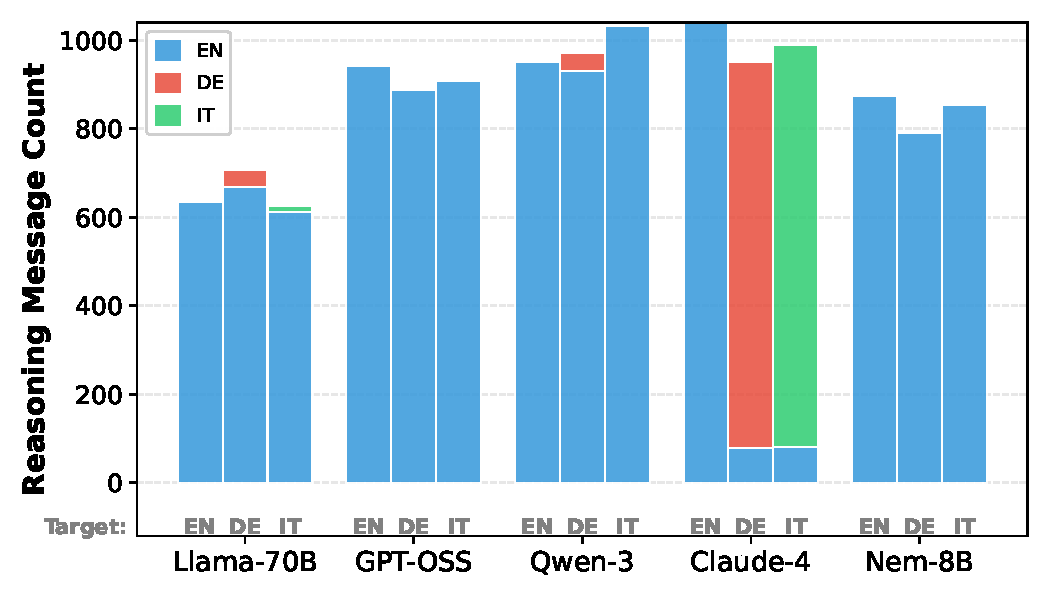
\includegraphics[width=\linewidth]{figures/language_distribution_reasoning_messages.pdf}
%         \caption{Language distribution in reasoning tokens}
%         \label{fig:lang_distribution_reasoning}
% \end{figure}

% \begin{table}[ht!]
% \centering
% \setlength{\tabcolsep}{4pt}
% \begin{tabular}{ll|ccc}
% & & \textbf{DE} & \textbf{EN} & \textbf{IT} \\
% \hline
% \multirow{2}{*}{Commercial} & completion & \cellcolor[rgb]{0.12,0.47,0.71}\textcolor{white}{1.00} & \cellcolor[rgb]{0.12,0.47,0.71}\textcolor{white}{1.00} & \cellcolor[rgb]{0.12,0.47,0.71}\textcolor{white}{1.00} \\
% & reasoning & \cellcolor[rgb]{0.99,0.75,0.44}\textcolor{black}{0.84} & \cellcolor[rgb]{0.12,0.47,0.71}\textcolor{white}{1.00} & \cellcolor[rgb]{0.99,0.75,0.44}\textcolor{black}{0.84} \\
% \hline
% \multirow{2}{*}{Open-weight} & completion & \cellcolor[rgb]{0.99,0.75,0.44}\textcolor{black}{0.94} & \cellcolor[rgb]{0.12,0.47,0.71}\textcolor{white}{1.00} & \cellcolor[rgb]{0.99,0.75,0.44}\textcolor{black}{0.87} \\
% & reasoning & \cellcolor[rgb]{0.40,0.15,0.28}\textcolor{white}{0.06} & \cellcolor[rgb]{0.12,0.47,0.71}\textcolor{white}{1.00} & \cellcolor[rgb]{0.40,0.15,0.28}\textcolor{white}{0.03} \\
% \end{tabular}
% \caption{Language consistency in reasoning tokens}
% \label{tab:lang_consistency}
%     % \vspace{-1.0em}
% \end{table}


\begin{figure}[ht!]
    \centering
    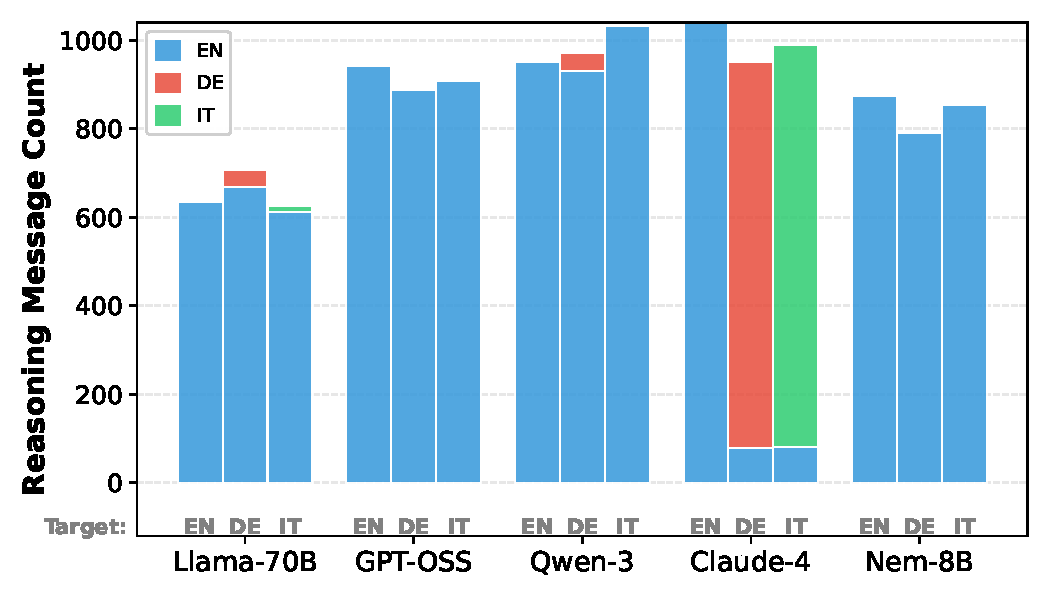
\includegraphics[width=\linewidth]{figures/language_distribution_reasoning_messages.pdf}
            \caption{Language distribution in reasoning tokens}
        \label{fig:lang_distribution_reasoning}
    
    \vspace{1em}
    
    \setlength{\tabcolsep}{4pt}
    \begin{tabular}{ll|ccc}
    & & \textbf{DE} & \textbf{EN} & \textbf{IT} \\
    \hline
    \multirow{2}{*}{Commercial} & completion & \cellcolor[rgb]{0.12,0.47,0.71}\textcolor{white}{1.00} & \cellcolor[rgb]{0.12,0.47,0.71}\textcolor{white}{1.00} & \cellcolor[rgb]{0.12,0.47,0.71}\textcolor{white}{1.00} \\
    & reasoning & \cellcolor[rgb]{0.99,0.75,0.44}\textcolor{black}{0.84} & \cellcolor[rgb]{0.12,0.47,0.71}\textcolor{white}{1.00} & \cellcolor[rgb]{0.99,0.75,0.44}\textcolor{black}{0.84} \\
    \hline
    \multirow{2}{*}{Open-weight} & completion & \cellcolor[rgb]{0.99,0.75,0.44}\textcolor{black}{0.94} & \cellcolor[rgb]{0.12,0.47,0.71}\textcolor{white}{1.00} & \cellcolor[rgb]{0.99,0.75,0.44}\textcolor{black}{0.87} \\
    & reasoning & \cellcolor[rgb]{0.40,0.15,0.28}\textcolor{white}{0.06} & \cellcolor[rgb]{0.12,0.47,0.71}\textcolor{white}{1.00} & \cellcolor[rgb]{0.40,0.15,0.28}\textcolor{white}{0.03} \\
    \end{tabular}
    
    \caption{Language consistency in reasoning tokens}
    \label{fig:lang_analysis}
        \vspace{-1.2em}
\end{figure}

        
% \begin{figure}[ht!]
%     \centering
    
%     % --- First Figure ---
%     \begin{subfigure}{\linewidth}
%         \centering
%         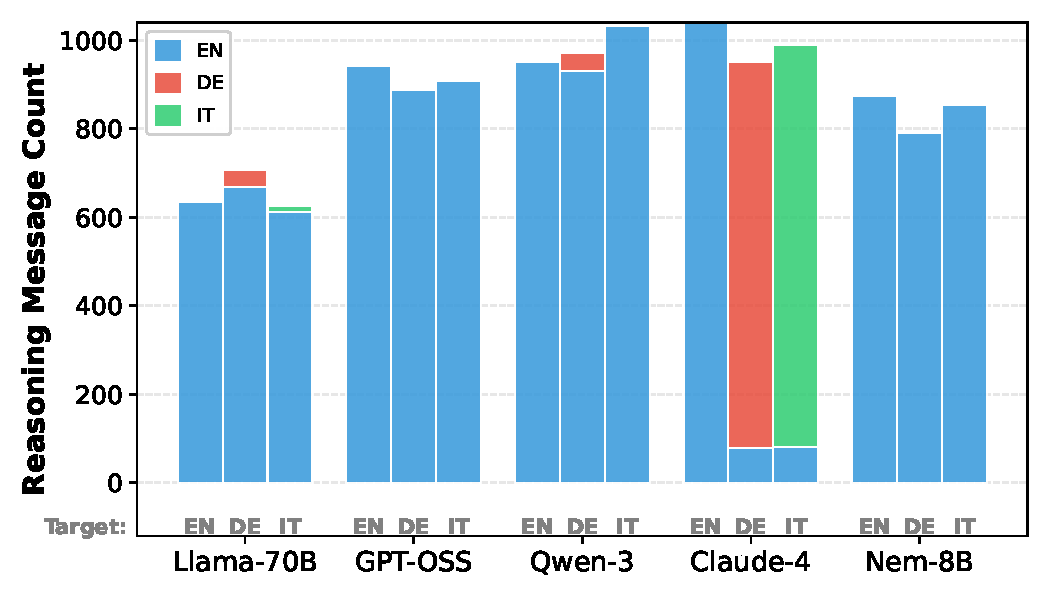
\includegraphics[width=\linewidth]{figures/language_distribution_reasoning_messages.pdf}
%         \caption{Language distribution in reasoning tokens}
%         \label{fig:lang_distribution_reasoning}
%     \end{subfigure}
    
%     % \vspace{-0.9em} % Adds vertical space between the two plots

%     % --- Second Figure ---
%     \begin{subfigure}{\linewidth}
%         \centering
%         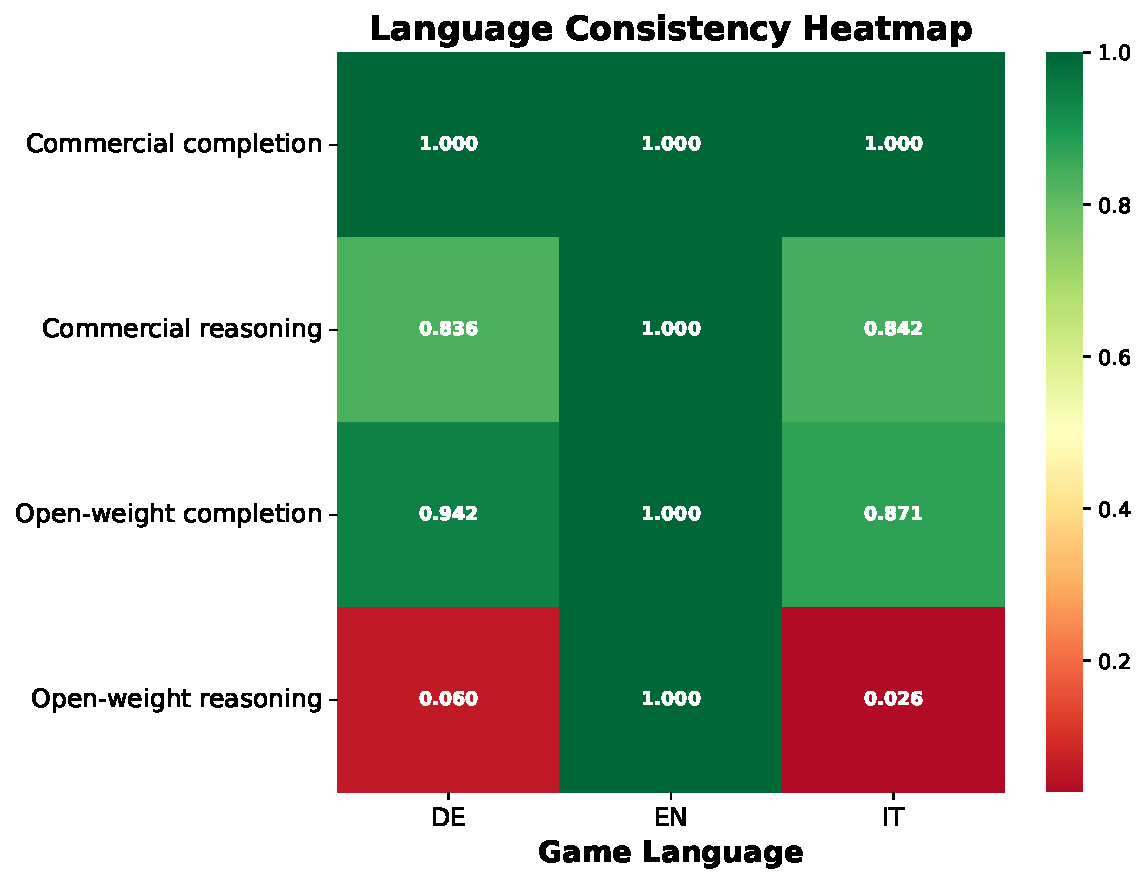
\includegraphics[width=\linewidth]{figures/mean_consistency_rates_heatmap.pdf}
%         \caption{Language consistency across model types (open-weight and commercial) for both completion and reasoning tokens.}
%         \label{fig:language_consistency_heatmap}
%     \end{subfigure}

%     % --- Main caption for the entire figure ---
%     \caption{Analysis of language use in model outputs, showing distribution in reasoning messages (a) and cross-model type language consistency (b).}
%     \label{fig:language_analysis_combined}
%     \vspace{-1.2em}
% \end{figure}



We ran a language detection script to analyse the reasoning message of the models. The results are presented in Figure~\ref{fig:lang_distribution_reasoning}\footnote{Note: \textit{GPT-5} models do not return reasoning tokens, thus they are excluded from further analysis}. We clearly see that all open-weight models mostly generate reasoning tokens in English, whereas \textit{Claude-4} ``thinks'' in the respective language of the task, consistently across all three of them. In Figure~\ref{fig:lang_analysis}, we provide a heat map showing language consistency (whether the language of the message matches the target language) across \textit{completion} and \textit{reasoning} tokens. 



We can clearly see that \textit{Claude-4} (the only commercial model in the analysis) exhibits consistency in both completion and reasoning tokens. Open-weight models retain consistency in completion tokens (thus, abiding by the formatting rules as each game requires prefixes in the respective language), but fail to do so with reasoning tokens for German and Italian versions of the games. Thus, we can conclude that \textbf{open-weight models do not maintain language consistency in their reasoning processes across multilingual tasks}.




\textbf{RQ3}: \textit{Do models demonstrate strategic adaptation over multiple turns, or merely surface-level pattern matching creating an illusion of thinking?}



We look at the first-turn reasoning tokens and detect certain states where the thinking process changes into. The states are detected using lexical cues in reasoning tokens, e.g. ``maybe/could'': \texttt{PROPOSE}; ``but/however'': \texttt{UNDERMINE}, etc. Then, we model these states as walks on a finite-state machine (see Appendix~\ref{sec:cyclic_analysis}) and compute two diagnostics: (i) number of segments (plan restarts/restructuring), and (ii) cycle edge ratio (within-segment looping). 
Good-performing models should resolve plans in fewer segments and cycles because to have more goal-oriented planning and execution of it. Performance shows non-linear relationships: \textbf{minimal segment counts correlate with improved outcomes}, while moderate additions yield unclear results. \textbf{Commercial models achieve competitive scores with lower cycle ratios} and tighter clustering; open-weight models show higher ratios with greater variance, suggesting that additional cycles do not reliably translate into performance gains.


\begin{figure}[ht!]
    \centering
    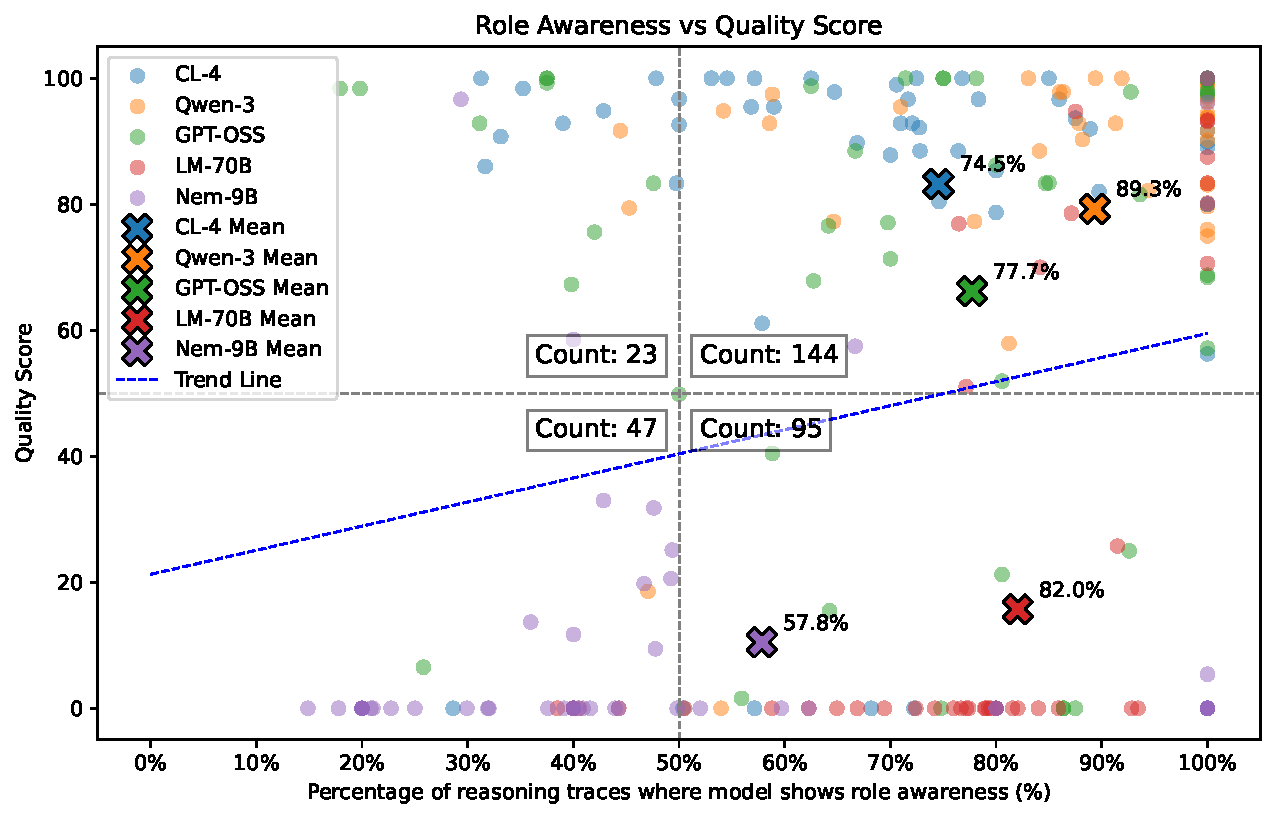
\includegraphics[width=\linewidth]{figures/role_awareness_vs_quality_score.pdf}
        \caption{Reasoning traces where the model displays both awareness of their own another player's role}
        \label{fig:role_awareness}
        \vspace{-1.2em}
\end{figure}


% \begin{figure}[ht!]
%     \centering
%     \begin{subfigure}{\linewidth}
%         \centering
%         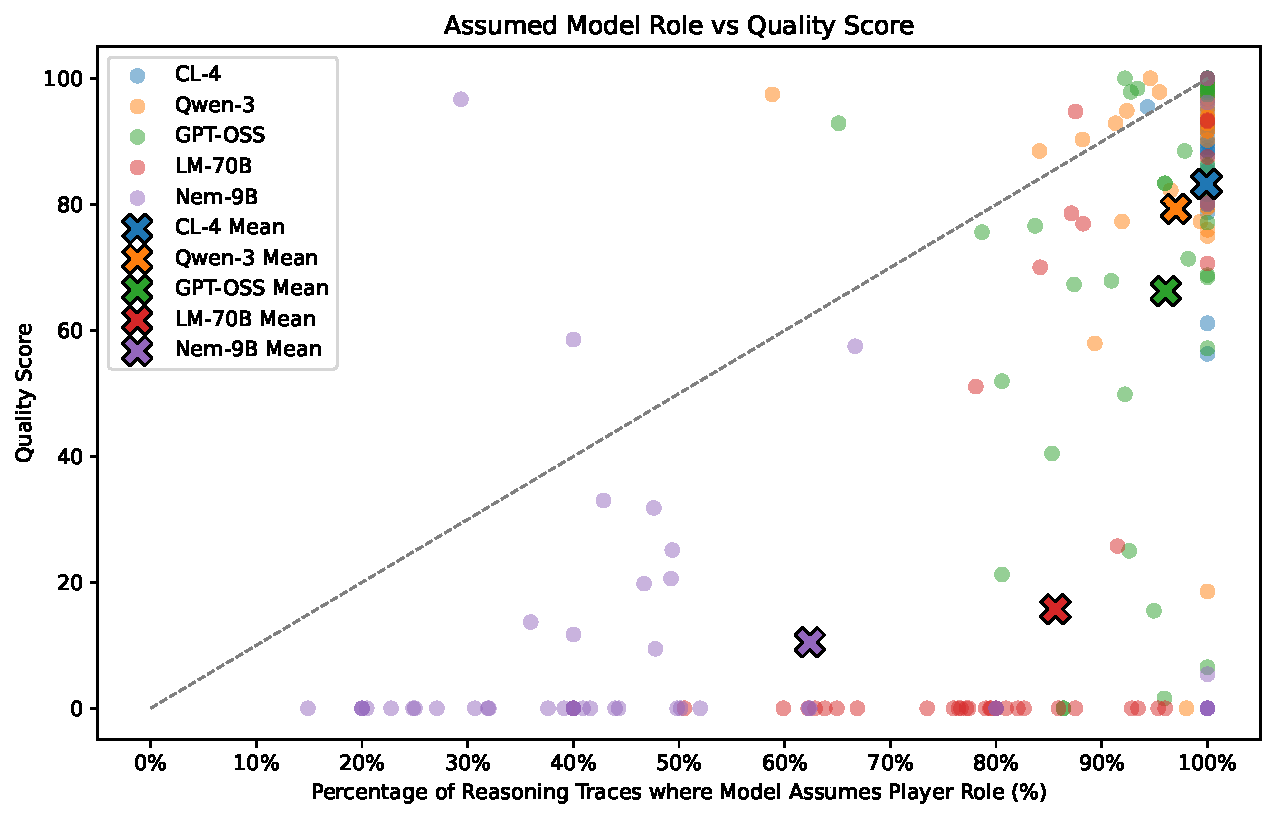
\includegraphics[width=\linewidth]{figures/author_role_vs_quality_score.pdf}
%         \caption{Percentage of reasoning traces where the model assumes a player role, as opposed to an assistant/helper role, plotted \textit{vs.} quality score.}
%     \label{fig:assumed_role}
%     \end{subfigure}
%     \hfill
%     \begin{subfigure}{\linewidth}
%         \centering
%         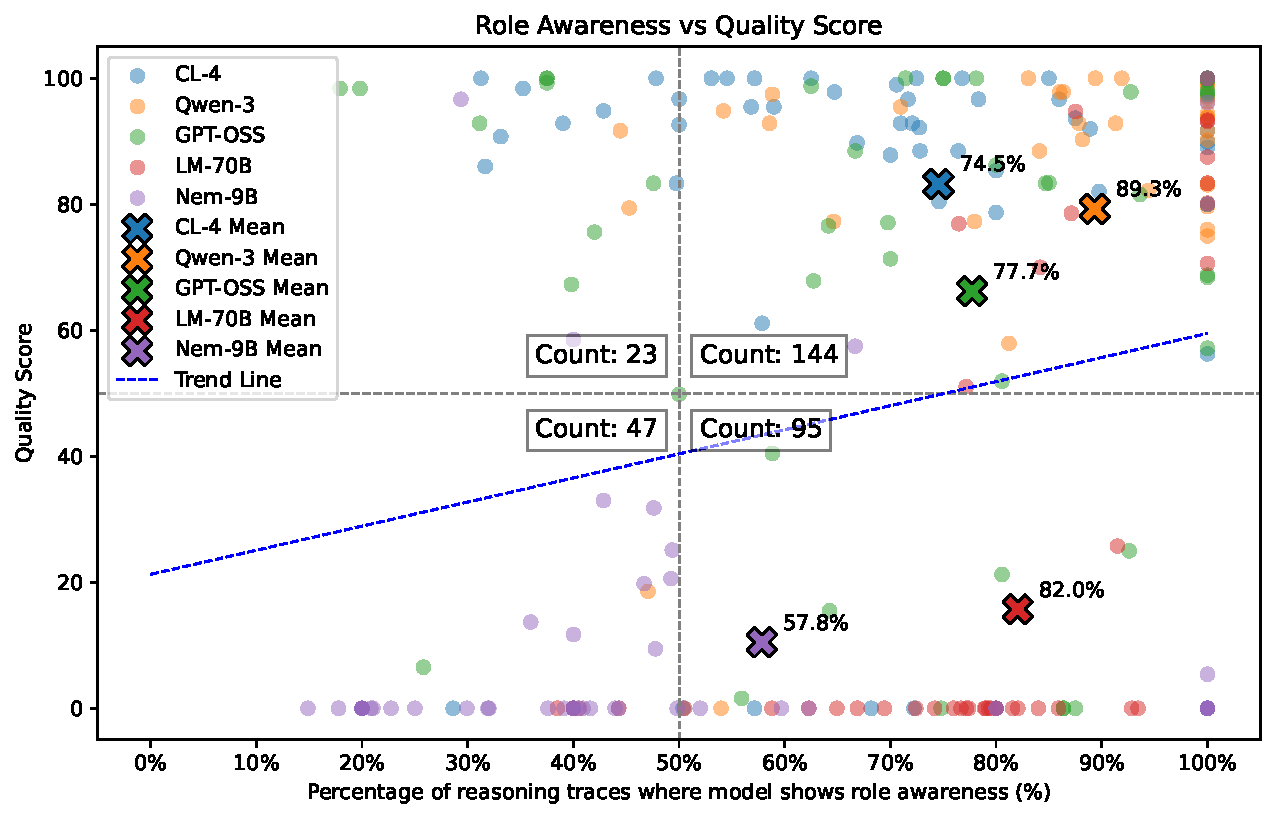
\includegraphics[width=\linewidth]{figures/role_awareness_vs_quality_score.pdf}
%         \caption{Percentage of reasoning traces where the model displays both awareness of their own player role \textit{and} of another player, plotted \textit{vs.} quality score.}
%         \label{fig:role_awareness}
%     \end{subfigure}
%     \caption{Plots of the models' self awareness (a) and self awareness combined with counterpart awareness (b) compared to achieved quality scores. Filled crosses show the mean values for each model.}
%     \label{fig:role_plots}
% \end{figure}

% \textbf{RQ4}: \textit{Do reasoning traces display that models are aware of both their own role and that of their counterpart, and how does this affect performance?}

Since the games prompt the model to be active agents, we analyse the reasoning traces for both awareness of their own player role (whether the model helping or advising somebody else, or actively playing the game itself) and of the partner (mention of any other agentic participant). The results given in Figure~\ref{fig:role_awareness} are obtained from the same LLM-based analysis (see Appendix~\ref{sec:llm-based_reasoning_analysis}). \textit{Qwen-3} shows the highest role awareness with an average of 89.3\%, followed by Llama-70B with 82.0\%, GPT-OSS with 77.7\%, Claude-4 with 74.5\%, and, lastly, Nemotron-9B with 57.8\%.
% Naturally, the mean percentages for all models are somewhat lower than those for assuming a player role, with 74.5\% for Claude-4, 89.3\% for Qwen-3, 77.7\% for GPT-OSS, 82.0\% for Llama-70B, and 57.8\% for Nemotron-9B.

Of all games with a quality score over $50$, 144 (46.6\% of games) show role awareness in over 50\% of reasoning traces, and only $23$ in under 50\%. Of the games with a quality score below $50$, 95 (30.7\%) show higher and 47 (15.2\%) lower role awareness. This indicates that \textbf{awareness of both one's own role and the existence of a counterpart are prerequisites for consistently high scores.}

% . Using LLM-based analysis (see \ref{sec:llm-based_reasoning_analysis}, we determined whether the model assumes a `player' role in each thinking trace of a total of 309 game transcripts. Complementary, models sometimes also take the role of an `assistant' helping a `user' who they assume to be playing the game. Fig.~\ref{fig:assumed_role} shows the percentage of traces written from an active player's perspective on the x-axis, and the quality score achieved in the respective games on the y-axis. While Claude-4, Qwen-3 and GPT-OSS assume an active role in the virtually all reasoning traces (with 99.9\%, 97.0\% and 96.0\%, respectively) and achieve high scores on average, Llama-70B and Nemotron-9B show lower percentages of 85.6\% and 62.4\% and much lower scores.

% An overwhelming majority of 95.15\% of all data points are below the dotted main diagonal, meaning that models rarely reach a quality score higher than the percentage of traces where they assume an active `player' role. It thus appears that \textbf{assuming an active role is a premise for a successful game,} but does by no means guarantee it.

% Additionally, fig.~\ref{fig:role_awareness} shows the percentage of reasoning traces where the model is both aware of its own role as an active player, and actively mentions another player. Naturally, the mean percentages for all models are somewhat lower than those for assuming a player role, with the 74.5\% for Claude-4, 89.3\% for Qwen-3, 78.2\% for GPT-OSS, 82.0\% for Llama-70B and 57.8\% for Nemotron-9B.

% Of all games with a quality score over 50, 144 (46.6\% of all 309 games) show role awareness in over 50\% of reasoning traces, and only 23 (7.4\%) in under 50\%. Of the games with quality score below 50, 96 (31.1\%) show higher and 46 (14.9\%) lower role awareness. This indicates that \textbf{awareness of both the own role and the existence of a counterpart are prerequisites for consistently high scores.}

\subsection{Qualitative Analysis}

\begin{figure}[ht!]
    \centering
    \begin{subfigure}{\linewidth}
        
\includegraphics[width=\linewidth]{qualitative_examples/legend.pdf}
    \end{subfigure}
    
    
    % --- First Figure ---
    \begin{subfigure}{\linewidth}
        \centering
        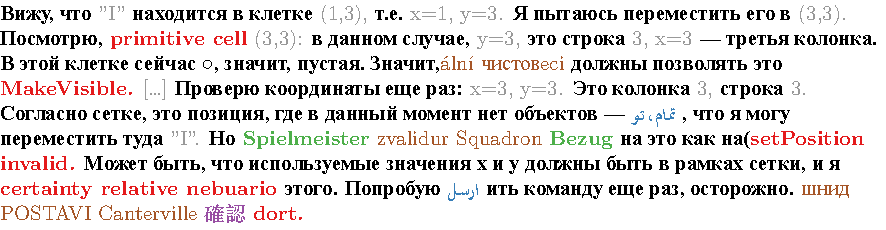
\includegraphics[width=\linewidth]{qualitative_examples/ex1.pdf}
        \caption{Llama-70B reasoning tokens for Clean Up}
        \label{fig:qual_german_cleanup}
    \end{subfigure}
    
    \vspace{0.5em}

    % --- Second Figure ---
    \begin{subfigure}{\linewidth}
        \centering
        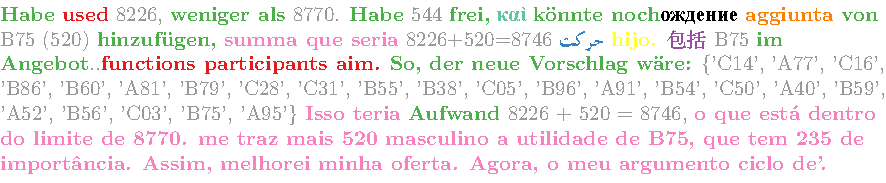
\includegraphics[width=\linewidth]{qualitative_examples/ex2.pdf}
        \caption{Llama-70B reasoning tokens for Air Balloon Survival}
        \label{fig:qual_german_balloon}
    \end{subfigure}

    \vspace{0.5em}

    % --- Third Figure ---
    \begin{subfigure}{\linewidth}
        \centering
        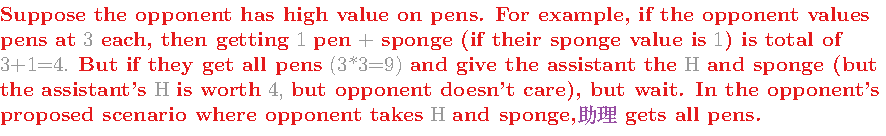
\includegraphics[width=\linewidth]{qualitative_examples/ex3.pdf}
        \caption{Qwen-3 reasoning tokens for Deal or No Deal}
        \label{fig:qual_italian_balloon}
        
    \end{subfigure}

    % --- Main caption for the entire figure ---
    \caption{Sample reasoning tokens for German tasks}
    \label{fig:qualitative_examples}
    \vspace{-1.2em}
\end{figure}

We provide qualitative samples in Figure~\ref{fig:qualitative_examples} from German task for reasoning tokens generated by \textit{Qwen-3} and \textit{Llama-70B} (distilled from Deepseek-R1). The top example shows how languages are interchangeably used, with Russian being the common one. It starts with: \foreignlanguage{russian}{Вижу, что} "I" \foreignlanguage{russian}{находится в клетке (1,3) ... Я пытаюсь переместить его в (3,3). Посмотрю,} primitive cell (3,3) \foreignlanguage{russian}{... В этой клетке сейчас $\circ$, значит, пустая.}, which translates to \textit{I can see that there is ``I'' in cell (1,3) ... and I try to move it  to (3,3) ... I look ... in this cell there is} $\circ$, \textit{meaning it is empty}.

The middle example shows how the model reasons about its choices and weights and tries to calculate what it means to consider one of them, and interchangeably uses eight languages.

The bottom example's reasoning is about modelling the opponent where the roles are confused because it refers to an ``assistant'' (\begin{CJK*}{UTF8}{gbsn}助理\end{CJK*}). But the actual task is for the assistant to act as the user, and the opponent is simulated.





\section{Conclusion}

We conducted the first comprehensive study systematically investigating the impact of reasoning on performance in multilingual negotiation tasks. 
Our work examines the trade-offs between computational cost and negotiation effectiveness, assesses the linguistic consistency of reasoning processes, and probes the depth of strategic adaptation in English, German, and Italian. Our findings reveal that test-time scaling is a powerful and costly tool: it significantly enhances negotiation performance, yet demands substantial additional compute. 
Open-weight models almost exclusively switch to English for internal reasoning, even when performing tasks in German or Italian, while leading commercial models maintain language consistency between reasoning and outputs. Our results further suggest that reasoning enables genuine strategic adaptation rather than simply pattern matching. The observed improvements in handling complex rules, making value-based decisions, and achieving collaborative outcomes point to deeper problem-solving unlocked when models ``think out loud'' before acting. 
Future work should extend this investigation to broader dialogue games, more diverse languages, and emerging models to chart the path toward AI agents that are versatile negotiators.


\section*{Limitations}

The first limitation is about the scope of negotiation tasks. Some researchers also employed other dialogue games that we did not include in this study, as there are many similarities among games and the measures they assess. Another limitation is the choice of languages for analysis, which are three European languages that are also high-resource languages. The primary reason for considering only the defined dialogue games and languages is that including more games or languages would result in a higher number of model results, thereby increasing the overall cost of the study. Another limitation is the exclusion of models from both commercial and open-source ones. As explained above, such decisions would exceed the budget for such a study. Given the obtained results regarding switching languages, it is evident that most models lack natural reasoning aspects, and utilising such models in real-world applications would bring its own set of challenges and limitations. For use cases that involve cultural or language-specific concepts or aspects, it can not be guaranteed that they will be well-understood in English (as most languages switch to it).

\section*{Ethical Considerations}

Using paid proprietary APIs with underlying models about which little is known (training data, model architecture) in academic research is less than ideal. Currently, the models tested here support reasoning modes, either on or off (except for GPT-OSS-120B and Deepseek-v3.1). We hope that open models will include more controls over reasoning aspects and catch up soon in terms of general performance. Deploying such language agents in society has considerable risks. As mentioned in the Related Work, such agents exhibit asymmetric behaviours in negotiations and may expose users to unfaithful actions.

%\bibliography{anthology,custom}
% Custom bibliography entries only
\bibliography{custom, anthology_0, anthology_1}

% \section*{Acknowledgments}




\appendix

\section{Additional Results}\label{sec:appendix_reamining_details}
\subfile{appendix/remainig_details}

\section{Deal or No Deal - Game Details}\label{sec:appendix_dond}
\subfile{dond/dond_appendix}


\section{Clean Up - Game Details}\label{sec:appendix_clean_up}
\subfile{clean_up/clean_up_appendix}

\section{Air Balloon Survival - Game Details}\label{sec:appendix_airballoon}
\subfile{air-balloon-survival/air_balloon_appendix}

\end{document}
